\documentclass[11pt,twocolumn,a4paper]{article}
\usepackage[top=0.72in,bottom=0.78in,left=0.68in,right=0.68in,columnsep=0.26in]{geometry}
\usepackage[T1]{fontenc}
\usepackage[utf8]{inputenc}
\usepackage{mathptmx}
\usepackage[scaled=0.92]{helvet}
\usepackage{microtype}
\usepackage{graphicx}
\usepackage{xcolor}
\usepackage{booktabs,tabularx,array,multirow}
\usepackage{needspace}
\usepackage{enumitem}
\newcolumntype{Y}{>{\raggedright\arraybackslash}X}
\usepackage{titlesec}
\usepackage[font=small,labelfont={bf,sf},textfont=it,labelsep=period,skip=3pt]{caption}
\usepackage{subcaption}
\usepackage{fancyhdr}
\usepackage{lastpage}
\usepackage{cite}
\usepackage{balance}
\usepackage[colorlinks=true,linkcolor=teal!60!black,citecolor=teal!60!black,urlcolor=teal!60!black]{hyperref}

\definecolor{navy}{HTML}{12263A}
\definecolor{teal}{HTML}{0E7C86}
\definecolor{amber}{HTML}{F4A261}
\definecolor{pale}{HTML}{EAF2F5}

% ---- headings ----
\titleformat{\section}{\sffamily\bfseries\small\color{navy}}{\thesection.}{0.5em}{\MakeUppercase}[{\color{teal}\titlerule[0.5pt]}]
\titleformat{\subsection}{\sffamily\bfseries\footnotesize\color{teal!70!black}}{\thesubsection}{0.5em}{}
\titlespacing*{\section}{0pt}{9pt}{4pt}
\titlespacing*{\subsection}{0pt}{6pt}{2pt}
\let\oldsubsection\subsection
\renewcommand{\subsection}{\Needspace*{4\baselineskip}\oldsubsection}
\let\oldsection\section
\renewcommand{\section}{\Needspace*{9\baselineskip}\oldsection}
\linespread{1.01}\selectfont
\setlength{\parskip}{0pt}
\setlength{\parindent}{9pt}
\setlist{nosep,leftmargin=1.1em,itemsep=1pt}
\renewcommand{\arraystretch}{1.12}
\setlength{\textfloatsep}{8pt plus 2pt minus 2pt}
\setlength{\floatsep}{7pt plus 2pt minus 2pt}
\setlength{\intextsep}{7pt plus 2pt minus 2pt}
\setlength{\dbltextfloatsep}{8pt plus 2pt minus 2pt}
\setlength{\abovecaptionskip}{3pt}

\renewcommand{\topfraction}{0.92}
\renewcommand{\dbltopfraction}{0.92}
\renewcommand{\bottomfraction}{0.3}
\renewcommand{\textfraction}{0.08}
\renewcommand{\floatpagefraction}{0.8}
\renewcommand{\dblfloatpagefraction}{0.8}
\setcounter{topnumber}{3}\setcounter{dbltopnumber}{2}\setcounter{totalnumber}{4}
\sloppy

\pagestyle{fancy}
\fancyhf{}
\renewcommand{\headrulewidth}{0.4pt}
\fancyhead[L]{\sffamily\scriptsize\color{navy}Segregation at the Point of Care: UX Critique and Grounded Design Proposal}
\fancyhead[R]{\sffamily\scriptsize\color{navy}Group M (Group 9) $\cdot$ FUX 2026--27}
\fancyfoot[C]{\sffamily\scriptsize\thepage\ / \pageref{LastPage}}
\fancypagestyle{first}{\fancyhf{}\renewcommand{\headrulewidth}{0pt}\fancyfoot[C]{\sffamily\scriptsize\thepage\ / \pageref{LastPage}}}

\newcommand{\hl}[1]{\textbf{\color{navy}#1}}
\newcommand{\figref}[1]{Fig.~\ref{#1}}
\newcommand{\tabref}[1]{Table~\ref{#1}}
\newcommand{\quoteS}[1]{\textit{``#1''}}

\begin{document}

% ================= TITLE BLOCK =================
\twocolumn[{%
\begin{center}
{\color{teal}\rule{\textwidth}{1.6pt}}\\[7pt]
{\sffamily\bfseries\fontsize{17}{20}\selectfont\color{navy} Segregation at the Point of Care}\\[3pt]
{\sffamily\fontsize{11.5}{14}\selectfont\color{navy} A UX Critique of Medical-Waste Handling at the Renovated IITGN Medical Centre\\ and a Literature-Grounded Design Proposal (AI-AMWS)}\\[7pt]
{\sffamily\small\textbf{Group M (Group 9)}}

\quad{\small Vipul Sunil Patil (22110189), Vraj Rajdeep (22110215), Gaurav Budhwani (22110085), Anish (24110041), Tanish (23110327), Smit Bambhroliya (24110345)}\\
{\small\itshape Foundations of User Experience (FUX), Semester 1, 2026--27 $\cdot$ Indian Institute of Technology Gandhinagar}\\
{\small Instructor: Prof.\ Nuno M.\ Guimar\~aes $\cdot$ Topic 10: Medical Waste Management}\\[5pt]
{\color{teal}\rule{\textwidth}{0.6pt}}
\end{center}
\vspace{-2pt}
\begin{center}
\begin{minipage}{0.94\textwidth}
\small\noindent{\sffamily\bfseries\color{navy}Abstract\,---\,}%
Bio-medical waste (BMW) segregation is a safety-critical task that depends on how well a physical environment supports busy, distracted people. The IITGN Medical Centre has recently undergone an interior and spatial renovation, providing an opportunity to study what a physical facility redesign does, and does not, change for clinical waste handling. This report presents an \emph{observation, critique and preliminary-design} exercise. We did not build a physical model or run an interventional clinical trial; we analyse what we documented across two on-site contextual inquiries (10 and 18~November~2026), identify systemic human-factors bottlenecks, and propose design evolutions justified by field evidence and published HCI and ergonomic literature. We mapped the renovated facility layout by hand, audited receptacles photographically without touching waste, sampled bin-to-wall contrast, and conducted semi-structured inquiries with clinical and operational staff under explicit verbal informed consent and strict participant anonymity. While the renovation introduced an organized 4-bin external balcony buffer rack, point-of-care receptacles inside patient rooms remain predominantly lidless, unlabelled, mismatched, unevenly loaded, and emptied reactively. Furthermore, staff rely on verbal briefings to bridge regulatory gaps, while surge management depends on an informal hybrid of evening support staffing (5:00--9:00~PM) and daytime on-demand phone calls. Reading these findings through Norman, Rasmussen and Reason, we derive six functional requirements and propose a staged trajectory: standardise first (Phase~0), introduce point-of-disposal guidance and fill sensing (Phase~1), and implement predictive forecasting and route optimization (Phase~2). We explicitly delineate what remains to be validated.\\[3pt]
{\sffamily\bfseries\color{navy}Keywords\,---\,}{\itshape bio-medical waste, safety-critical UX, signifiers, error prevention, healthcare ergonomics, design critique}
\end{minipage}
\end{center}
\vspace{4pt}
}]
\thispagestyle{first}

% ================= 1 INTRODUCTION =================
\section{Introduction}
\subsection{Why bins are a safety interface}
Waste handling in a clinic is where infection control, occupational safety and environmental law meet. A needle in the wrong container injures a housekeeper; a contaminated item in a general bin leaves the regulated stream. The World Health Organization requires segregation at the point of generation \cite{who2014}, and India's Bio-Medical Waste Management (BMW) Rules, 2016 make colour-coded segregation a legal duty \cite{bmw2016}. Contaminated sharps are a documented source of occupational infection \cite{prusstun2005}, and reviews of Indian practice repeatedly point to weak segregation at source as a root problem \cite{datta2018,capoor2017}.

Segregation happens in seconds, while attention is on a patient. We therefore treat the bin as an \emph{interface}, not as furniture. Following Norman \cite{norman2013}, a good interface makes the correct action discoverable, gives feedback and lets errors be caught.

\subsection{Scope: what this report is, and is not}
The brief offers two directions. We follow \textbf{Direction~1}: take an existing artefact, here the waste-disposal system of the \emph{renovated} Medical Centre, explore its use, identify problems, suggest evolutions and be critical about the UX. Our suggested evolution (AI-AMWS) is a \emph{preliminary design}, in the brief's words an exercise in observation, ideation and preliminary design. Three boundaries are deliberate:
\begin{itemize}
\item \textbf{We did not build a prototype, train a model or test with users.} Doing so was not feasible in a clinical setting within the course, and would have needed approvals we do not have.
\item \textbf{We ground instead of test.} Each proposal is tied to a field observation and to cited research, and \tabref{tab:ground} states what each citation does and does not establish.
\item \textbf{We say what could be done and how it could be achieved,} not that it has been done. Where a claim is our judgement, we say so.
\end{itemize}

\subsection{Objectives and contributions}
\textbf{O1.} Document how the renovation changed the physical, visual and logistical context of disposal. \textbf{O2.} Identify breakdowns in affordance, signification, mapping, feedback and workflow, with photographic evidence. \textbf{O3.} Propose evolutions, compare them with simpler alternatives, and justify them from literature. \textbf{O4.} Reflect honestly on method limits. Our contributions are a field-grounded comparison with the baseline, a photo-based compliance checklist, a requirement set tied to HCI theory, a staged design proposal with alternatives, and an explicit evidence-grounding table.

% ================= 2 QUESTIONS =================
\section{Research Questions and Propositions}
\textbf{RQ1 (Spatial).} How did renovation change the placement of, and access to, receptacles? \textbf{RQ2 (Signification).} Do receptacles communicate category and correct use without verbal instruction? \textbf{RQ3 (Workflow).} How do generation, internal transfer and external collection work, and where do they fail? \textbf{RQ4 (Design).} Which evolutions are justified by evidence, and in what order should they be adopted?

Because we did not run a controlled study, we state our expectations as \emph{analytic propositions} to be examined against evidence, not as statistically tested hypotheses. \textbf{P1:} the renovation invested in the external buffer but not at the point of care, so interior receptacles will fall short of the buffer rack on the same simple checks (lid, colour, label). \textbf{P2:} reliance on verbal briefing signals a gulf of execution at the bin. \textbf{P3:} demand that staff describe as not clock-driven makes a fixed collection schedule and fixed bin sizes a poor fit. We treat P3 as plausible but thinly evidenced (one source, staff testimony). \textbf{P4:} guidance, feedback and capacity awareness at the point of disposal should reduce errors; this we can only argue from literature.

% ================= 3 BACKGROUND =================
\section{Background and Evidence Base}
\subsection{Regulatory context}
The BMW Rules 2016 prescribe containers per waste category \cite{bmw2016}. \tabref{tab:cpcb} lists the streams relevant to a clinic. Beyond colour, the Rules and their 2018 amendment require the biohazard symbol on containers, a barcode system on bags and containers, on-site pre-treatment of laboratory and microbiological waste, and a 48-hour limit on storing untreated waste \cite{bmw2016,bmw2018}. General waste falls under separate municipal rules \cite{swm2016}. Barcodes, symbols and pre-treatment cannot be judged from our photographs, so we report them as \emph{not verified}.
\begin{table}[!t]
\centering\footnotesize
\caption{Streams relevant to the Medical Centre. Black is not a BMW category.}\label{tab:cpcb}
\begin{tabularx}{\columnwidth}{@{}>{\bfseries}l Y@{}}
\toprule
Colour & Typical contents (BMW Rules 2016 \cite{bmw2016})\\\midrule
Yellow & Soiled cotton and dressings, anatomical waste, expired drugs\\
Red & Contaminated recyclable plastics: gloves, tubing, syringes without needles\\
White & Sharps (translucent, puncture-proof): needles, scalpels, blades\\
Blue & Glass and metallic implants (marked cardboard box)\\
Black & \emph{Outside the BMW Rules:} general or domestic-hazardous waste, municipal rules \cite{swm2016}\\
\bottomrule
\end{tabularx}
\end{table}

\subsection{Systemic risks of mis-segregation}
Errors propagate three ways. \emph{Occupational:} a needle in a soft bag injures whoever lifts it \cite{prusstun2005}. \emph{Infection control:} contaminated items in the general stream, or beside clean consumables, expose unprotected people \cite{who2014}. \emph{Environmental and legal:} each colour maps to a treatment route, so an item in the wrong bag meets the wrong process \cite{who2014,bmw2016}. A segregation error is rarely just a clinician's slip.

\subsection{HCI foundations}
\textbf{Norman's action cycle.} Breakdowns appear as a \emph{gulf of execution} (``which bin?'') or of \emph{evaluation} (``did that work?'') \cite{norman1986,norman2013}. \textbf{Rasmussen's SRK model.} Experienced staff act at the skill level, which is fast but slip-prone when attention is elsewhere; unfamiliar situations need explicit cues \cite{rasmussen1983}. \textbf{Reason's Swiss-cheese model.} Accidents occur when latent conditions (layout, labels, schedules) line up with active slips, so designers should add independent layers of defence rather than blame the last person \cite{reason1990,reason2000}.

\subsection{Evidence for the interventions we later propose}
We rely on five bodies of work. (i)~\emph{Nudges:} prompts placed at the moment of choice change behaviour without instruction \cite{thaler2008}. (ii)~\emph{Error-proofing (poka-yoke):} shape and constraint prevent wrong actions better than rules \cite{shingo1986}. (iii)~\emph{Alarm fatigue:} frequent low-value alerts are ignored, so signals must be rare and meaningful \cite{sendelbach2013,wickens2013}. (iv)~\emph{Colour vision and contrast:} colour-only coding excludes some users \cite{birch2012}, and WCAG recommends at least 3:1 contrast for non-text objects \cite{wcag2018}. (v)~\emph{Sensing and forecasting:} fill-level IoT is established in municipal waste \cite{medvedev2015}, while forecasting should begin with simple seasonal baselines before complex models \cite{hyndman2021,taylor2018}. Most audits, including the earlier study of this centre and ours, are retrospective snapshots; continuous sensing would show surges and drifts.

% ================= 4 METHOD =================
\section{Methodology}
\subsection{Design and sources}
We used a multi-visit comparative design. \emph{Primary data} were gathered across two fieldwork sessions at the renovated centre on 10 and 18~November~2026, triangulating clinical and operational perspectives. \emph{Secondary data} come from the documented baseline study of the pre-renovation facility by an earlier cohort of this course \cite{g8report}, provided as course reference material. It recorded approximately 100--150 daily visitors, 15 bins across five functional zones, and once-daily collection from three observation sessions (255 minutes total) and interviews with 5 nurses, 3 housekeeping staff, and 2 administrators. We reuse its descriptive findings strictly as historical baseline context, without replicating its specific measurements.

\subsection{Instruments}
\begin{itemize}
\item \textbf{Hand-drawn architectural floor plan} (\figref{fig:rawplan}), sketched during our first on-site walkthrough to map clinical zones, patient flow, and bin locations.
\item \textbf{Photographic audit} using mobile cameras, strictly restricted to waste receptacles, structural fixtures, and wall surfaces; no patients, clinical procedures, or human faces were photographed. From this audit we derived a \textbf{receptacle compliance checklist} (\tabref{tab:check}) and a \textbf{luminance-contrast sample} (\figref{fig:contrast}).
\item \textbf{Semi-structured contextual inquiries} conducted across two visits with facility personnel: (i)~Visit~1 (clinical perspective) with the \emph{Assistant Staff Nurse (N1)}, focusing on point-of-care clinical disposal, patient briefing practices, wall paint rationale, and perceived peak hours; (ii)~Visit~2 (operational perspective) with the \emph{Primary Waste Management Operator (P1)}, examining downstream segregation, transfer mechanics, dedicated shift staffing (including the 5:00~PM--9:00~PM support staff P2), and the external collection cadence.
\item \textbf{Contextual observation} of room-by-room hardware, waste accumulation levels, and the outdoor balcony buffer rack.
\end{itemize}

\subsection{Ethics and permission}
Nothing was touched, opened or moved. Photographs show equipment and physical surfaces only. For all on-site photographs, hand-drawn architectural floor plan sketches, and recorded audio interactions across both visits, explicit informed verbal consent was obtained from the respective healthcare and operational staff members present on-site. In strict accordance with academic research ethics, participant privacy, and institutional confidentiality mandates, all individual names, personal identifiers, and recording timestamps have been completely anonymized and redacted throughout this report. Individuals are designated strictly by functional role codes (\emph{Assistant Staff Nurse N1}, \emph{Primary Waste Operator P1}, \emph{Evening Support Staff P2}). Audio assets serve solely for empirical fact verification without direct attribution.

\subsection{Analysis}
We coded notes and photographs inductively into themes \cite{braun2006}, mapped themes to Norman's constructs, and evaluated the current setup with a scenario-based \emph{heuristic evaluation} \cite{nielsen1990,nielsen1994} using the authors as evaluators and an adapted severity scale (0--4) \cite{nielsen1993}. This is a heuristic evaluation, not a cognitive walkthrough.

\begin{figure}[!t]
\centering
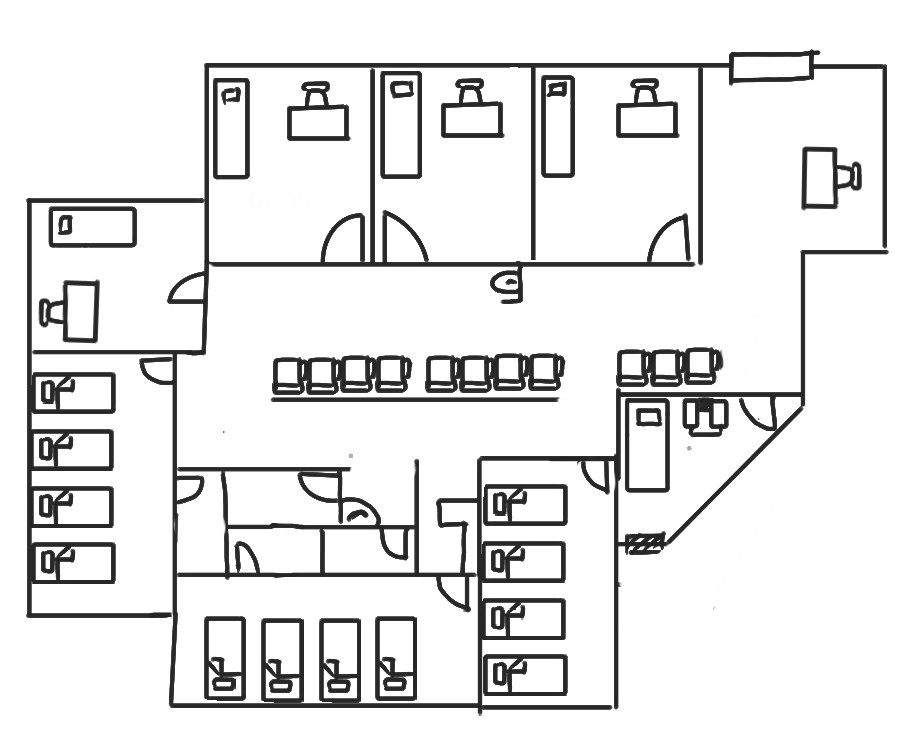
\includegraphics[width=0.95\columnwidth]{fig/plan_raw.jpg}
\caption{Hand-drawn floor plan of the renovated centre from the first walkthrough: central waiting lounge, three consultation cabins (north), dressing/minor-OT room (west), observation and sample areas (south and east).}\label{fig:rawplan}
\end{figure}

% ================= 5 FINDINGS =================
\section{Findings: The Renovated Medical Centre}
\subsection{F1. A renovation that stopped at the buffer rack}
During our initial walkthrough on 10~November~2026, we produced a hand-annotated architectural floor plan of the renovated clinic (\figref{fig:rawplan}) based on on-site observations. Asked whether bins were reconsidered during the facility renovation, staff replied: \quoteS{there were no excess reforms for dustbins, except for the outermost buffer dustbins}. The balcony rack (\figref{fig:buffer}) is done well: four lidded pedal bins in black, blue, red and yellow, each with a liner of matching colour, on a wheeled trolley. It is also the staging point where waste waits for the external and campus collection teams (F6). We use it as an \emph{internal benchmark}: the institution can specify and buy correct standard bins. Inside the clinic the picture differs (P1). Note that the stickers visible on the rack are brand marks, not category labels, so even here the category is carried by colour alone.

\begin{figure}[!ht]
\centering
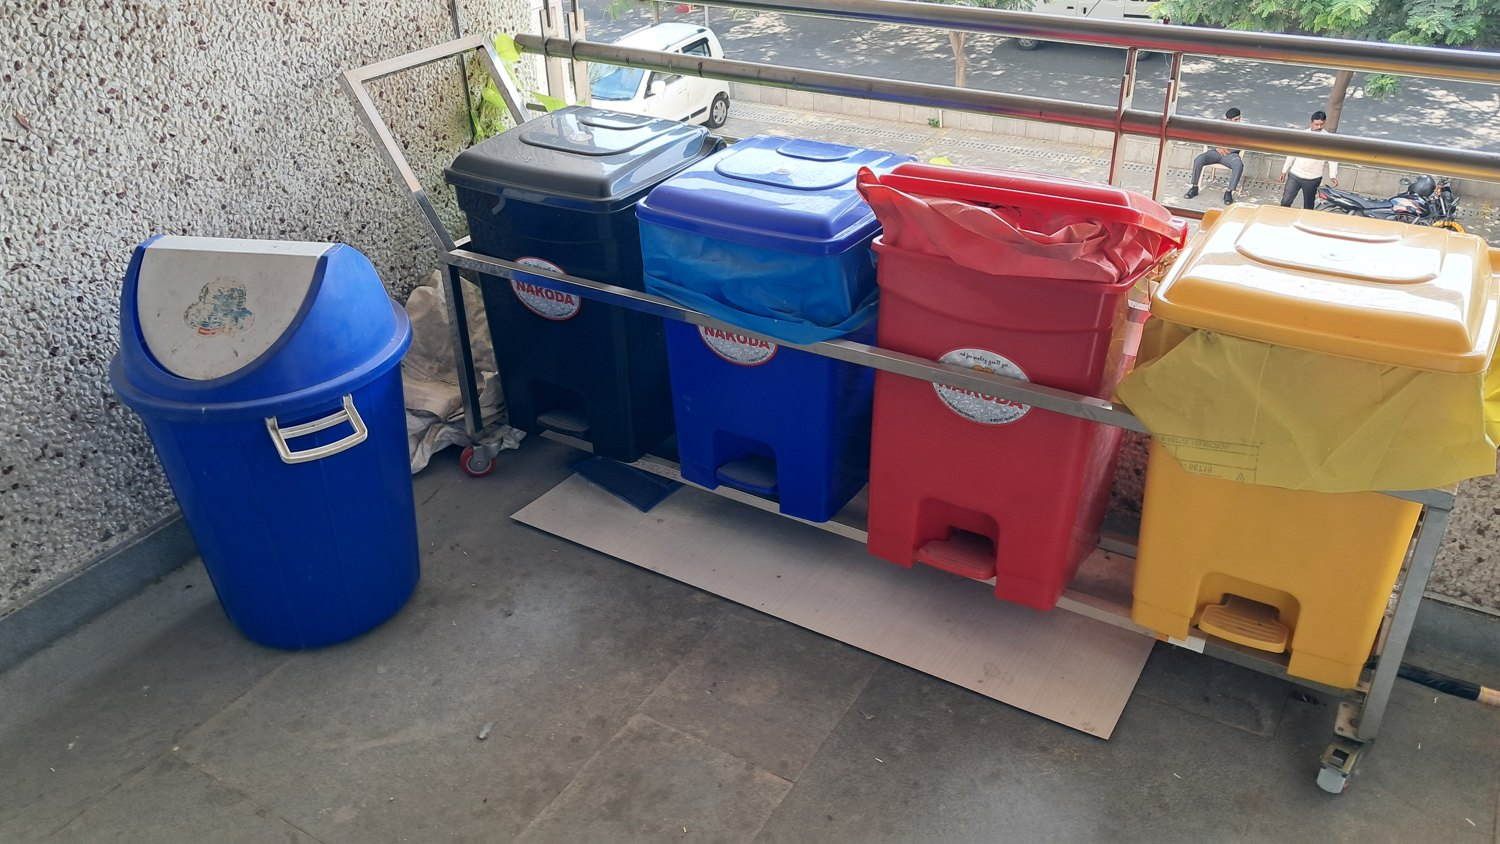
\includegraphics[width=\columnwidth]{fig/p_buffer2.jpg}
\caption{External balcony buffer rack: four pedal bins in standard colours with matching liners. The separate blue swing bin on the left sits outside the scheme.}\label{fig:buffer}
\end{figure}

\subsection{F2. Point-of-care receptacles are non-standard, unlabelled and unevenly full}
Under the sample-room counter (\figref{fig:overflow}) we found three open buckets: a red one holding syringe wrappers, one with an orange liner (orange, perhaps a faded red, is not a BMW colour) holding uncapped syringes, and a beige office bin holding blood-soiled cotton. None has a lid or a legible category label. The photograph also shows how \emph{unevenly} they are filled. Judged by eye, bucket~1 is heaped above its rim, bucket~2 is roughly three-quarters full and bucket~3 about a quarter full. Three receptacles in one corner, all in daily use, are at three different stages, and nothing signals this from the doorway. This is the on-site evidence for the capacity half of our proposal (Feature~B). In a procedure room (\figref{fig:contrast}a) a light-blue pedal bin carries a \emph{yellow} liner, beside open orange and blue buckets, chemical jugs and a yellow swing bin. Colour signifiers contradict each other: blue conventionally means glass, yellow soiled or anatomical waste.

\begin{figure}[!ht]
\centering
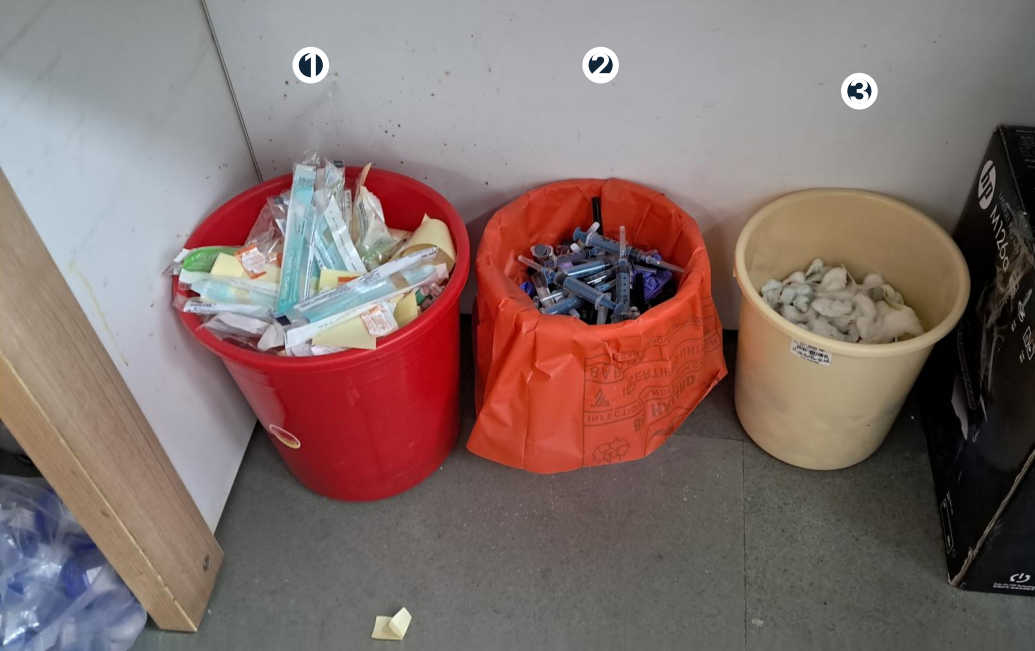
\includegraphics[width=\columnwidth]{fig/p_overflow_ann.png}
\caption{Sample-room counter. (1) Red bucket heaped above the rim with syringe wrappers; (2) orange-lined bucket, roughly three-quarters full of uncapped syringes; (3) beige bin, about a quarter full of blood-soiled cotton. Fill levels are visual estimates.}\label{fig:overflow}
\end{figure}

\subsection{F3. Mechanical affordances are broken}
A blue swing-top bin has a cracked flap lying sideways next to an open yellow bin containing soiled gauze (\figref{fig:evidence2}a). A domestic pedal bin with a grey lid and an orange liner stands among disinfectant cans (\figref{fig:evidence2}b). When a lid fails, the user either touches the container or leaves it open; both remove the barrier a bin should provide.

\begin{figure}[!ht]
\centering
\begin{subfigure}[t]{0.485\columnwidth}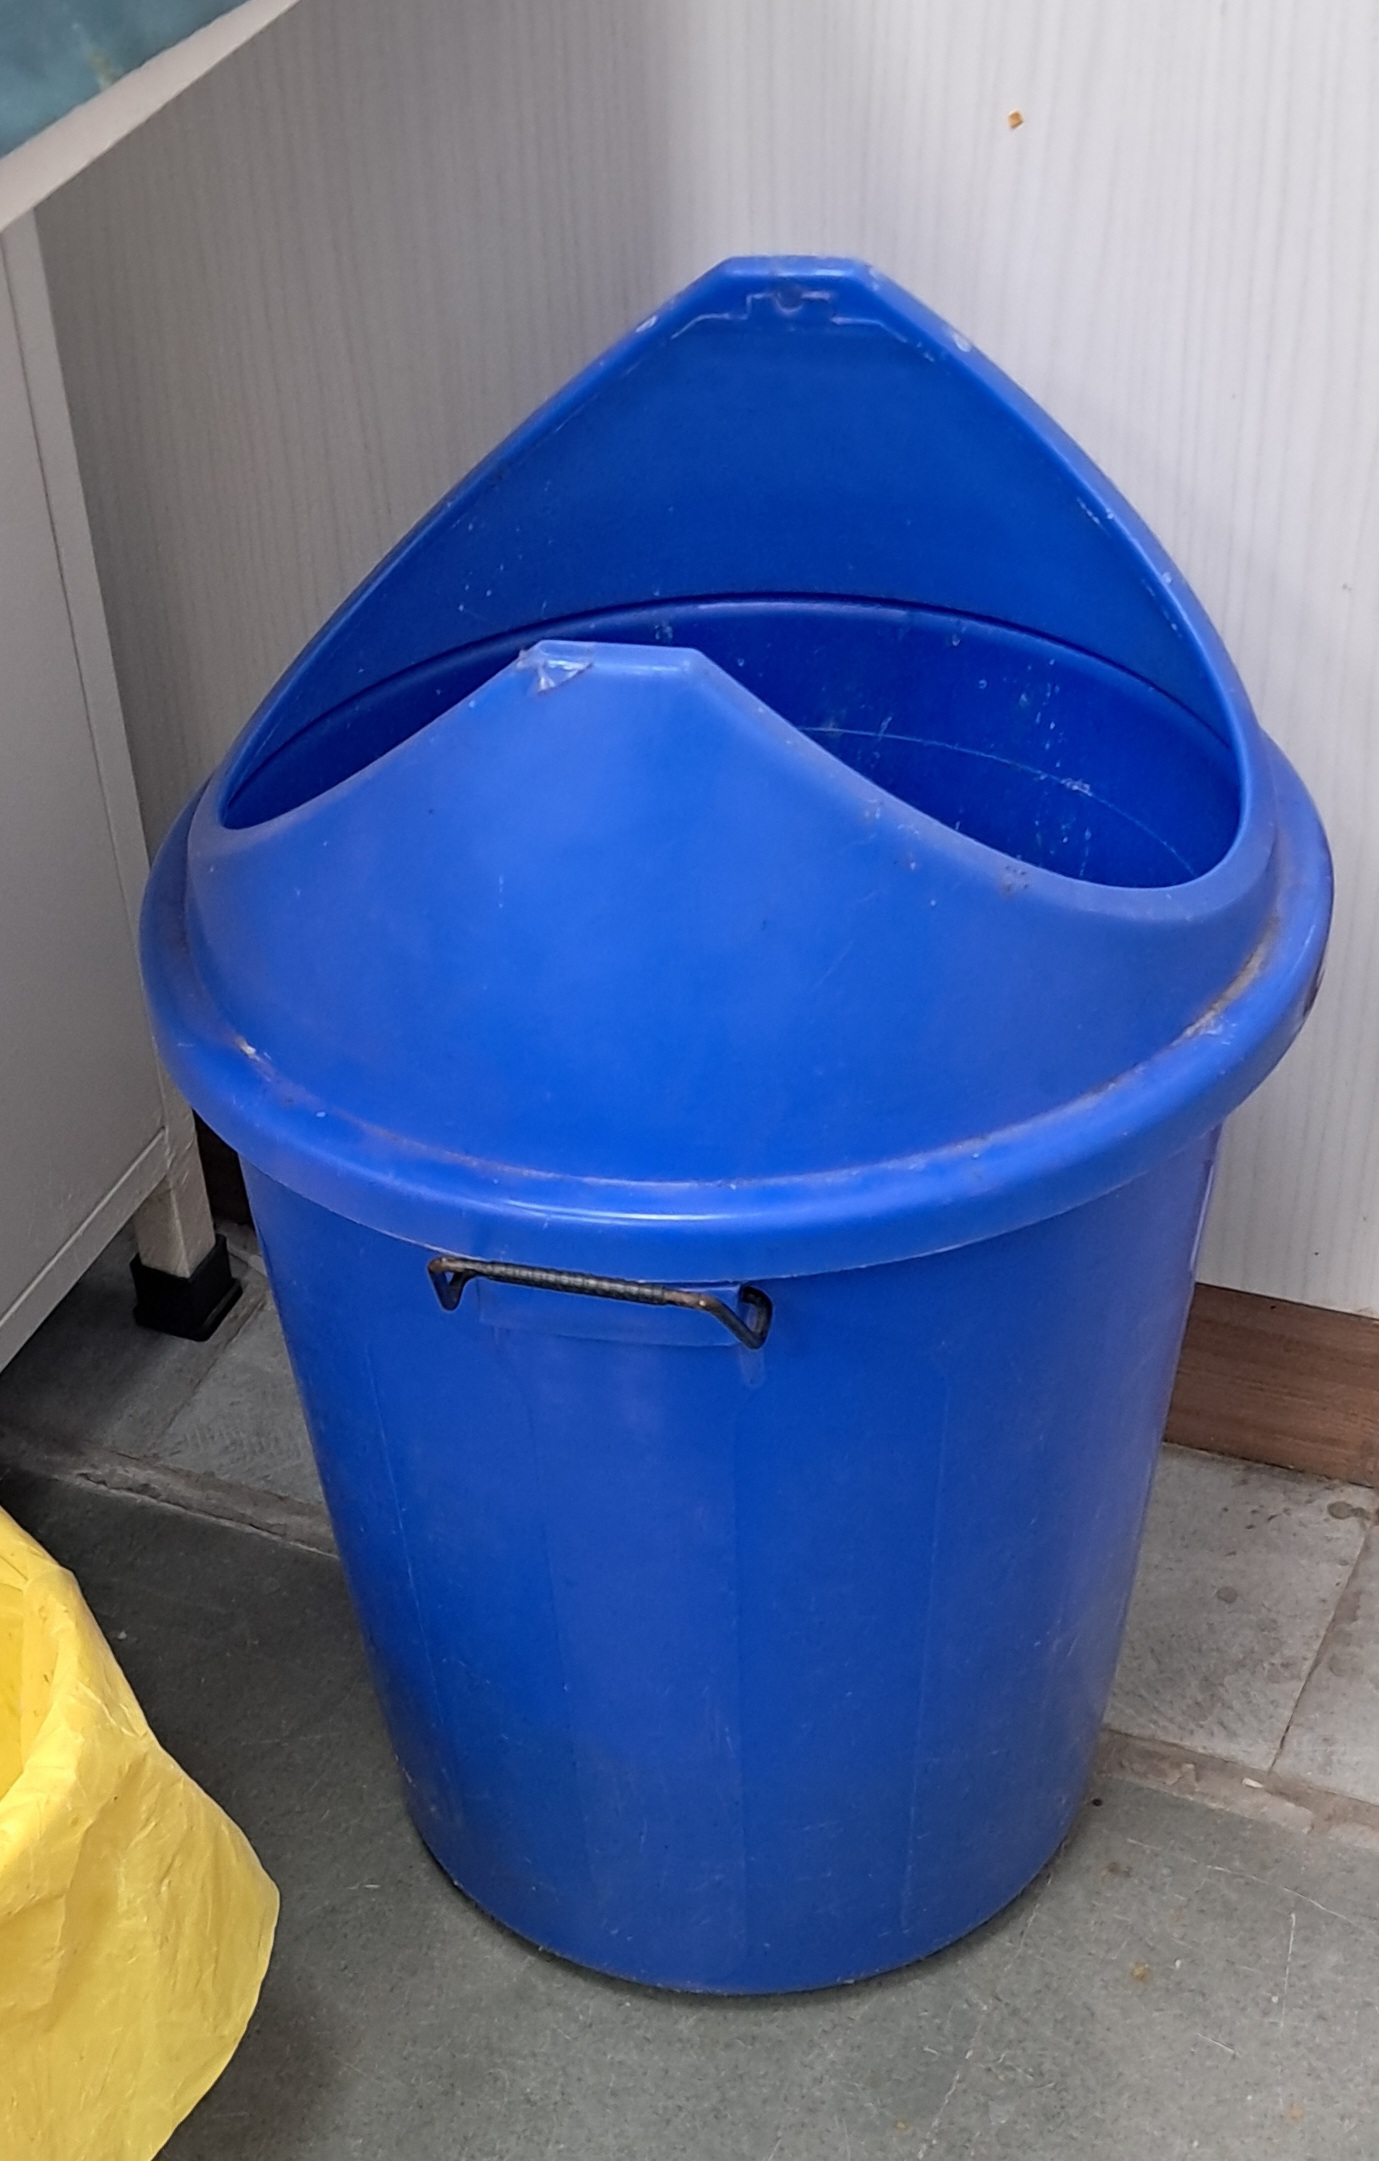
\includegraphics[width=\linewidth]{fig/p_broken.jpg}\caption{Cracked swing flap beside an open yellow bin.}\end{subfigure}\hfill
\begin{subfigure}[t]{0.485\columnwidth}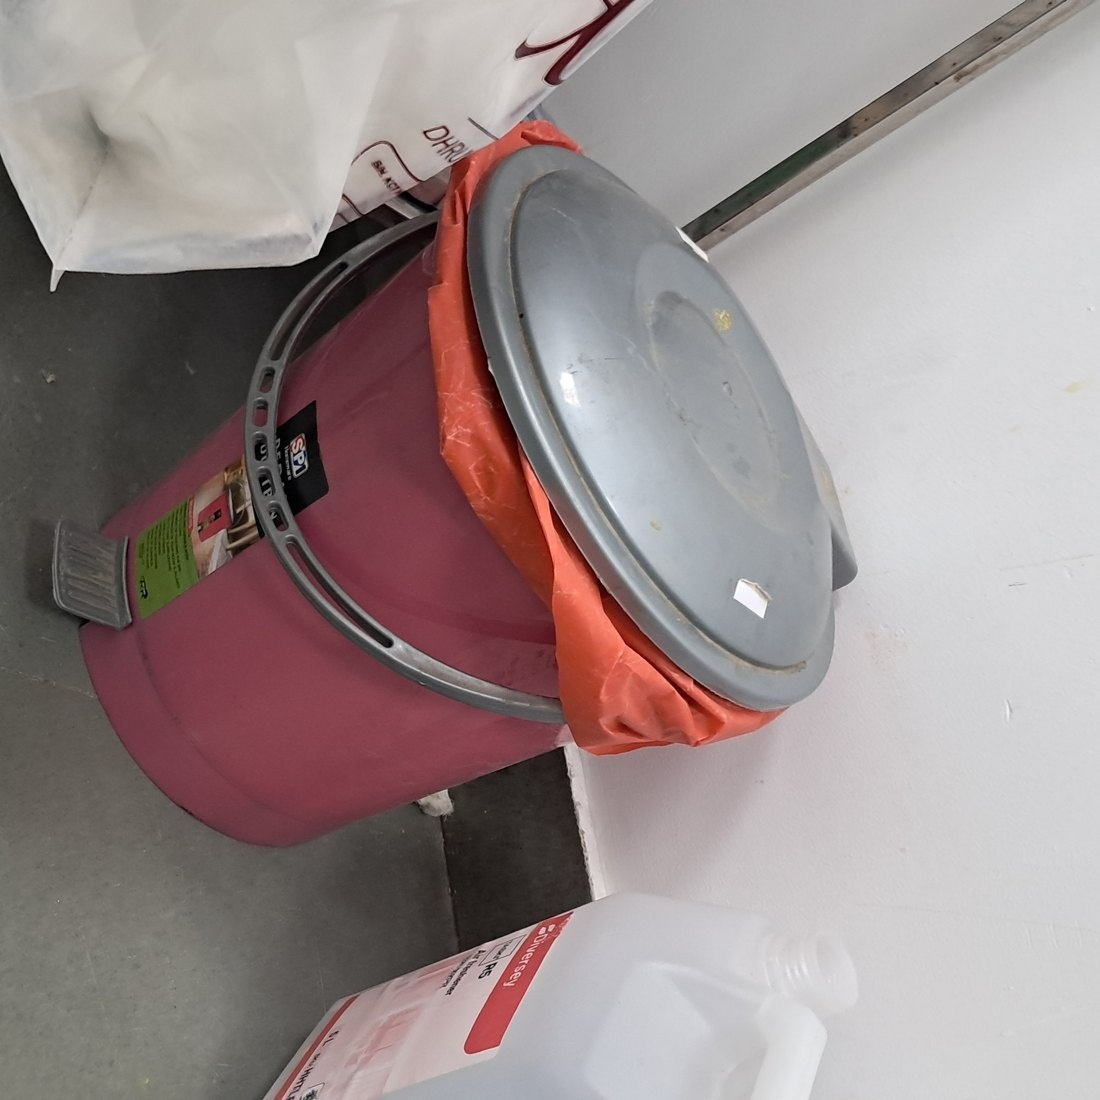
\includegraphics[width=\linewidth]{fig/p_pedal.jpg}\caption{Domestic pedal bin, orange liner, solvent cans.}\end{subfigure}
\caption{Broken or domestic hardware in a clinical space.}\label{fig:evidence2}
\end{figure}

\subsection{F3b. A simple compliance checklist from the photographs}
To give P1 some numbers, we scored every receptacle visible in our photographs on three observable checks (\tabref{tab:check}). This is a tally of photographed receptacles, \emph{not a census}, and it reflects our reading of the images.
\begin{table}[!ht]
\centering\footnotesize
\caption{Photo-based checklist: receptacles passing each check. ``Colour consistent'': container and liner use one BMW colour. Interior = sample room 3, procedure-room row 4, broken-flap photo 2, domestic bin 1. Barcode, biohazard symbol and pre-treatment: not verifiable from photographs.}\label{tab:check}
\begin{tabularx}{\columnwidth}{@{}>{\bfseries}p{1.9cm} c Y Y Y@{}}
\toprule
Location & n & Working lid & Colour consistent & Legible label\\\midrule
Balcony rack & 4 & 4 & 4 & 0\\
Interior rooms & 10 & 3 & 4 (1 n/a) & 0\\
\bottomrule
\end{tabularx}
\end{table}
Interior receptacles pass the lid check 3 times out of 10 and none shows a legible category label, against 4 of 4 lids on the rack. Under the working definitions above this supports P1, with the caveat that the sample is small and opportunistic.

\subsection{F4. Verbal briefing as a fragile workaround and CPCB adaptation}
Inquired regarding regulatory compliance and patient guidance, clinical staff (Assistant Staff Nurse N1) noted that institutional policy aligns with national CPCB guidelines (White for sharps, Black for general solid waste). However, enforcing the complete five-category CPCB set across every clinical and examination room was evaluated as \quoteS{too restrictive} and cumbersome given tight room spaces and fast patient turnover. Instead, rooms deploy common-purpose and primary-category receptacles. Clinical staff bridge this gap through manual intervention: \quoteS{before a patient comes or when admitted, staff have a communication regarding which dustbin they should use}. This reliance on verbal briefings confirms P2: an anxious, distracted, or acutely unwell patient cannot be expected to recall a verbal rule; the information needs to live on the object itself. Downstream, Primary Waste Operator P1 manages sorting via an operational 4-colour schedule (Blue for sharps, Black for chemical and pharmaceutical waste, Yellow for anatomical/soiled waste, Red for contaminated plastics), alongside a dedicated exterior black bin for unusable or expired medicines.

\subsection{F5. The wall-paint fix: helpful, but only for some bins}
Management told us they asked painters for a light colour \quoteS{so that the dustbins get highlighted}, after patient feedback that bins were not visible. This is a sound, evidence-driven decision. We tested it by sampling luminance contrast between the repainted wall and four bins in one procedure-room photograph with the WCAG relative-luminance ratio \cite{wcag2018} (\figref{fig:contrast}). Dark or saturated bins stand out: the blue bucket reaches 7.5:1 and the light-blue pedal bin 5.0:1. The red bucket only just clears 3:1 (3.2:1), and the \emph{yellow} bin, the colour for soiled and anatomical waste, is lowest at 1.9:1. So the paint helps dark bins most and the most routine hazardous stream least, and the pale wall also makes the row's mismatch plain. These values come from one phone photograph with automatic exposure, so they are indicative only.

\begin{figure*}[!t]
\centering
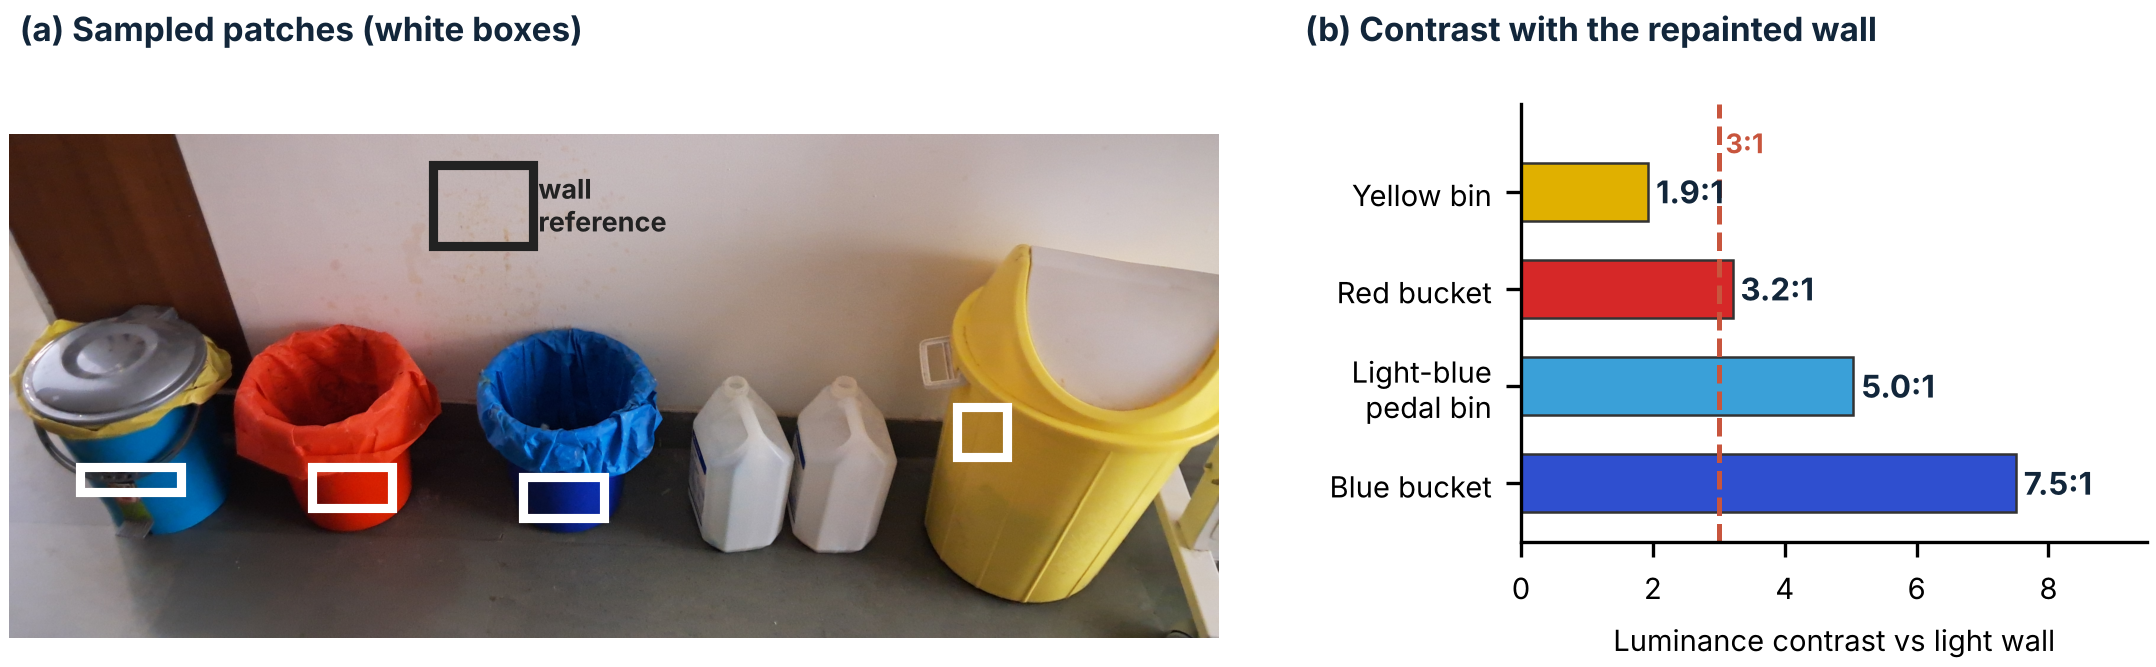
\includegraphics[width=0.80\textwidth]{fig/fig_contrast.png}
\caption{Procedure-room lineup and the effect of the repainted wall. (a) Photograph with sampled patches; the light-blue pedal bin on the left carries a yellow liner. (b) WCAG luminance contrast of each bin against the wall (single photograph; indicative).}\label{fig:contrast}
\end{figure*}

\subsection{F6. Unpredictable surges, hybrid staffing and a multi-tiered logistics chain}
Staff noted that clinical procedure volume is erratic: \quoteS{there are no consistent peak hours}, with the Minor OT and dressing areas filling fastest while receptacles are \quoteS{not sized consistently}. Through multi-stakeholder inquiry across both visits, we identified a hybrid operational model:
\begin{enumerate}
\item \emph{Scheduled evening surge coverage:} To manage the late-afternoon rush and emergency load, the facility deployed an evening co-worker (Support Staff P2) who works alongside Operator P1 from 5:00~PM to 9:00~PM, conducting scheduled collection rounds and transfers.
\item \emph{Daytime reactive on-demand calling:} Prior to 5:00~PM, or whenever unscheduled daytime procedures cause sudden overflows in the Minor OT or Triage, clinical staff telephone housekeeping on demand.
\end{enumerate}
Internal waste is carried to the exterior balcony buffer rack. External collection follows two distinct cadences: municipal general waste is cleared daily by the campus sanitation crew, whereas regulated bio-medical waste on the balcony rack is collected by an authorized external BMW contractor \emph{every three days} (a 72-hour cycle). \figref{fig:overflow} illustrates the vulnerability of this reactive daytime model: one bucket heaped, one nearly full, and one barely used, with no warning until clinical staff notice and phone. This confirms P3 and underscores the need for real-time capacity monitoring and automated dispatch.

\subsection{F7. Clean and contaminated items share space}
The wider view of the sample-room counter (\figref{fig:adjacent}a) shows the buckets directly below a rack of clean sample tubes and beside a printer cart. Sharps-bearing waste near clean consumables is a cross-contamination risk that bin design alone cannot solve; it needs placement away from clean work surfaces. We also photographed the staff pantry (\figref{fig:adjacent}b), which shows that a general-waste stream exists in the same building and needs its own clearly separate receptacle.

\begin{figure}[!ht]
\centering
\begin{subfigure}[t]{0.485\columnwidth}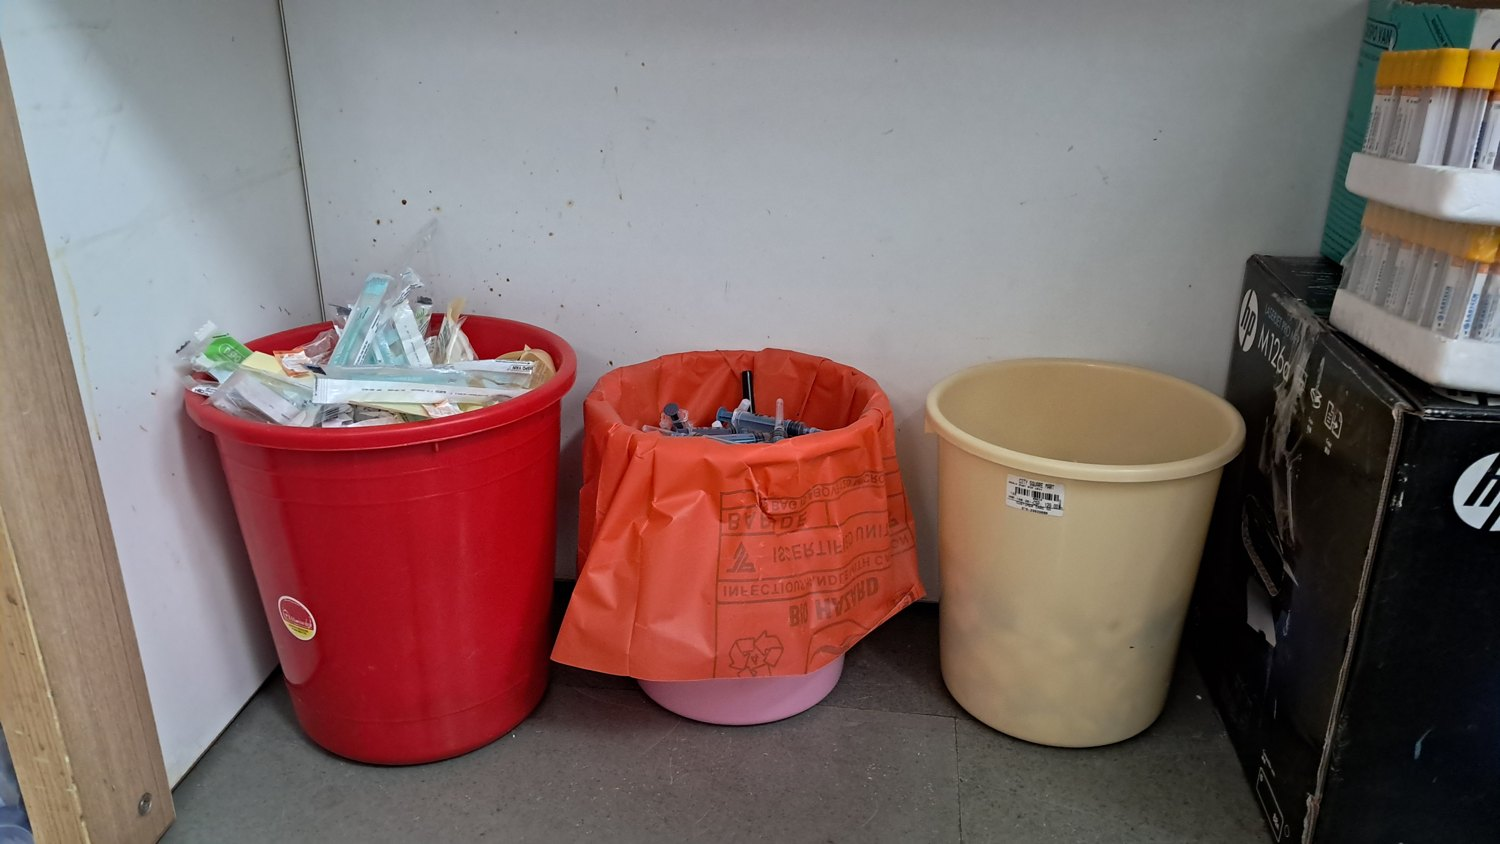
\includegraphics[width=\linewidth,height=2.3cm]{fig/p_cross.jpg}\caption{Waste beside clean tubes and a printer cart.}\end{subfigure}\hfill
\begin{subfigure}[t]{0.485\columnwidth}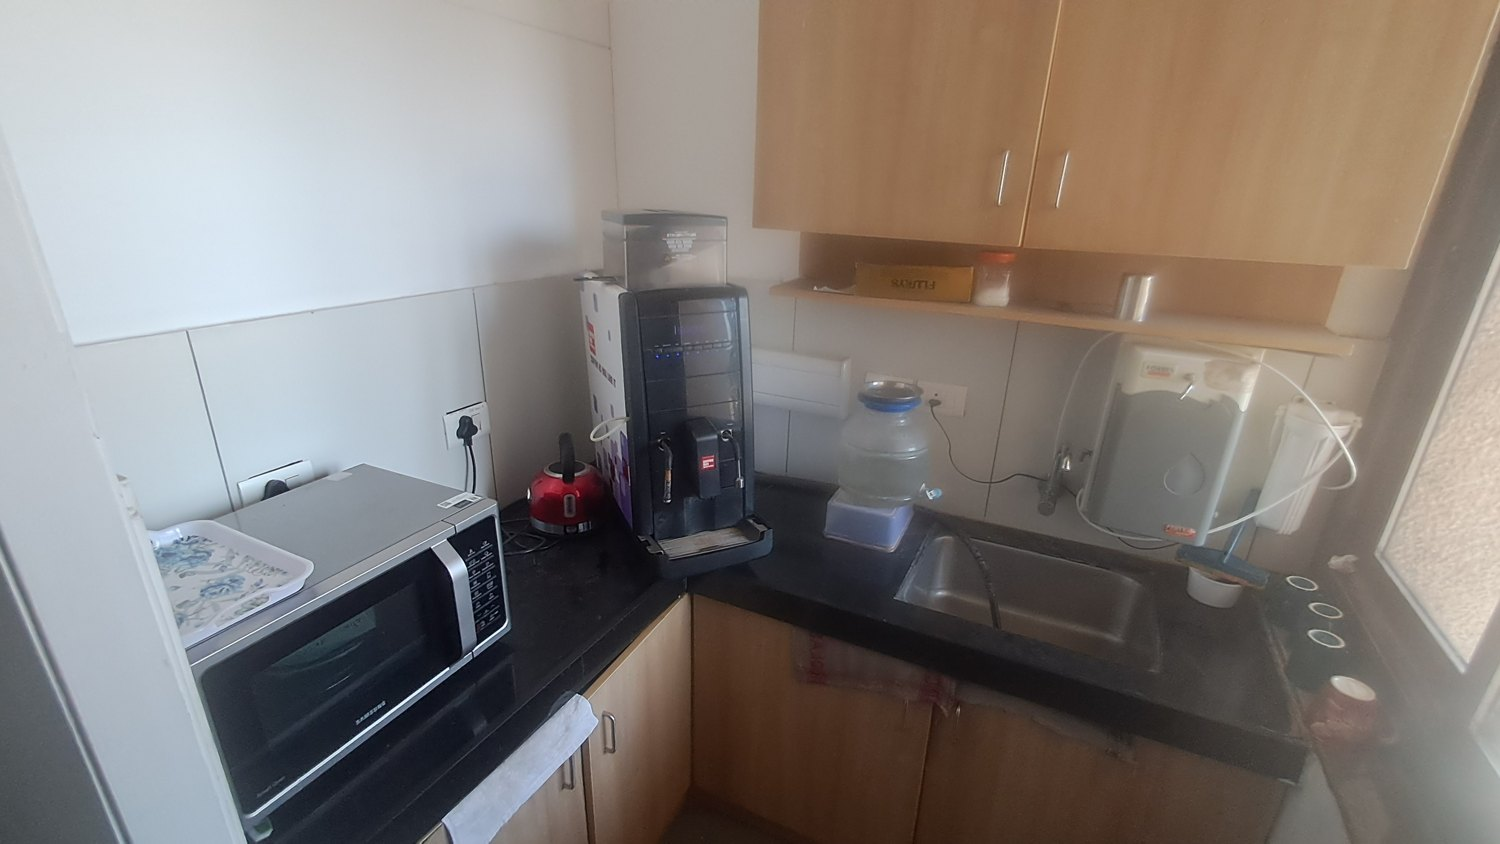
\includegraphics[width=\linewidth,height=2.3cm]{fig/p_pantry.jpg}\caption{Staff pantry: a general-waste stream.}\end{subfigure}
\caption{Adjacency problems: contaminated and clean items, clinical and food waste.}\label{fig:adjacent}
\end{figure}

\subsection{Comparison with the pre-renovation baseline}
\tabref{tab:compare} sets the baseline beside what we observed. We avoid numerical claims for the renovated site that we did not measure. Our plan marks 10 bins (\figref{fig:plans}A); this is a marked subset, \emph{not} a full inventory, so it is not comparable with the baseline's 15.
\begin{table*}[!t]
\centering\footnotesize
\caption{Pre-renovation baseline \cite{g8report} versus renovated centre (field visits, Nov 2026).}\label{tab:compare}
\begin{tabularx}{\textwidth}{@{}>{\bfseries}p{2.6cm} Y Y Y@{}}
\toprule
Dimension & Pre-renovation (documented baseline) & Renovated centre (our observation) & Net change\\\midrule
Layout and reach & Cramped rooms; bins in corners and behind furniture; visitors and staff mixed in corridors. & Renovated facility with wider corridors and partitions; 10 bins marked on our hand-drawn plan (not a census), several in corners or behind counters. & Space improved; point-of-care bin ergonomics not planned.\\
Colour and labels & Mostly CPCB colours but faded or handwritten labels and bag--bin mismatch. & Rack standard; interior mixed colours, verbal briefings substitute for labels, yellow liner in light-blue bin. & Worse inside, better outside.\\
Visual contrast & Cream/beige walls and tiles reduced visibility. & Lighter walls chosen to highlight bins. In one photograph, blue bins reach 7.5:1 but yellow only 1.9:1. & Partial: helps dark bins.\\
Mechanisms & Pedal and swing bins in use. & Open buckets; one broken flap; domestic bin. & No evidence of improvement.\\
Feedback & None beyond peeking into the bag. & None. & Unchanged.\\
Capacity & Afternoon overfill in the treatment room. & Minor OT fills fastest; unevenly sized and filled bins; no consistent daytime peak. & Unchanged.\\
Collection & Once-daily internal sweep; external pickup each morning. & Hybrid: on-demand daytime calls + evening staff (5--9 PM); balcony buffer; campus daily general sweep, 72-h external BMW pickup. & New buffer stage; evening support added; daytime remains reactive.\\
\bottomrule
\end{tabularx}
\end{table*}

% ================= 6 CRITICAL ANALYSIS =================
\section{Critical Analysis}
\subsection{Through Norman's lens}
\textbf{Gulf of execution.} With no legible category marks and mixed colours, users must recall a rule from memory or a briefing. \textbf{Gulf of evaluation.} No bin says whether a drop was correct, so errors are silent. \textbf{Mapping.} Bins sit in corners rather than beside the cot, trolley or sample chair. \textbf{Constraints.} Open buckets accept anything.

\subsection{Through SRK and Swiss cheese}
Under pressure staff act at the \emph{skill} level and choose the nearest open container, which unlabelled open buckets permit. Occasional users (patients, students) act at the \emph{knowledge} level and need cues they do not get. In Reason's terms the latent holes are visible in our photographs: mismatched liners, absent labels, broken lids, uneven capacity, a call-based schedule. An active slip passes through all of them because no layer is independent (\figref{fig:swiss}).
\begin{figure}[!t]
\centering
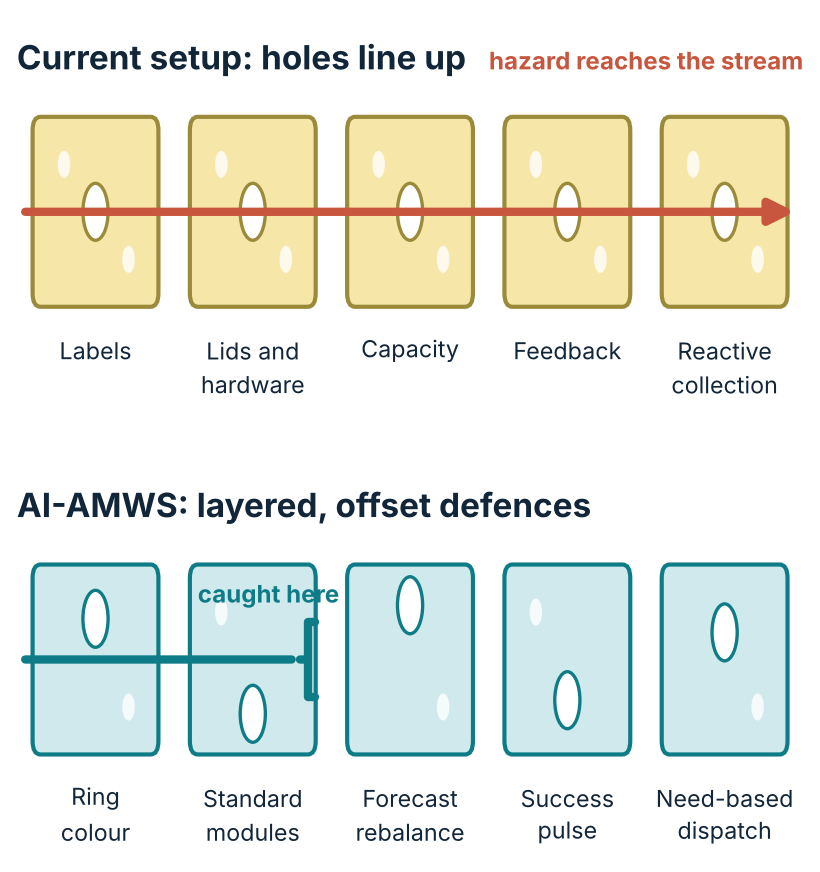
\includegraphics[width=0.8\columnwidth]{fig/fig_swiss.png}
\caption{Defence layers (after Reason \cite{reason1990}). Current setup: holes align. Proposed: added layers with offset holes.}\label{fig:swiss}
\end{figure}

\subsection{Stakeholders}
We infer, rather than elicit, how groups think. Clinicians choose the nearest open container by habit; patients follow a verbal rule if they remember it; housekeepers respond to calls without early warning; administrators have invested in the buffer rack and paint after complaints. No patient or housekeeper was interviewed directly, so this is a limitation of Direction~1's ``real users'' aim (Section~9).

\subsection{Heuristic evaluation of the current setup}
\tabref{tab:heur} rates the current setup on all ten of Nielsen's heuristics \cite{nielsen1994} (0 = none, 4 = catastrophic). These are the \emph{authors'} ratings; the method recommends several independent evaluators \cite{nielsen1990}, which we did not have.
\begin{table*}[!t]
\centering\footnotesize
\caption{Heuristic evaluation of the current setup (authors' ratings) and proposed response.}\label{tab:heur}
\begin{tabularx}{\textwidth}{@{}>{\bfseries}p{3.3cm} Y c Y@{}}
\toprule
Heuristic & Evidence in current setup & Sev. & Proposed response\\\midrule
Visibility of system status & No fill or success signal; overflow found by looking (\figref{fig:overflow}). & 3 & Ambient capacity glow; success pulse; alert at 75\% fill.\\
Match with real world & Blue bin with yellow liner contradicts BMW colour meaning. & 4 & Colour fixed to the module, not the liner.\\
User control and freedom & A wrong drop cannot be undone once bagged; no way to flag it. & 2 & Mismatch flag and audit log so a correction can follow.\\
Consistency and standards & Mixed domestic and clinical bins; inconsistent colours. & 3 & One modular family; same layout in every room.\\
Error prevention & Open buckets accept anything; wrappers by uncapped syringes. & 4 & Shaped apertures, sharps interlock \cite{shingo1986}.\\
Recognition over recall & Staff and patients rely on verbal briefing. & 4 & Colour and pictogram appear at the aperture on approach.\\
Flexibility and efficiency & Cannot resize bins when a room surges. & 3 & Module swap guided by fill velocity.\\
Aesthetic and minimalist design & Not an issue; light walls help. & 1 & Light backplate; little on-bin text.\\
Help recognise, diagnose, recover from errors & Nothing tells the user a drop was wrong or why. & 3 & Amber double-flash with reason shown in the app.\\
Help and documentation & Posters absent or unnoticed. & 2 & Pictogram on backplate; QR to a one-page guide.\\
\bottomrule
\end{tabularx}
\end{table*}

\subsection{Derived requirements}
\textbf{R1} Put the rule on the object (F2, F4). \textbf{R2} Give feedback on success and on near-capacity (F2, F6). \textbf{R3} Standardise hardware: lids, pedals, fixed liner colours (F2, F3). \textbf{R4} Match capacity to demand (F2, F6). \textbf{R5} Dispatch by need, not by call (F6). \textbf{R6} Place stations by workflow and away from clean work surfaces (F7, \figref{fig:plans}).

% ================= 7 DESIGN =================
\section{Suggested Evolution: AI-AMWS}
\subsection{Alternatives considered, and a staged path}
A critic can fairly say that standard bins, liners and labels would fix much of what we saw. We agree, so we compare options before proposing anything (\tabref{tab:alt}). Cost tiers are relative; we obtained no quotes.
\begin{table*}[!t]
\centering\footnotesize
\caption{Design alternatives and the staged path we suggest.}\label{tab:alt}
\begin{tabularx}{\textwidth}{@{}>{\bfseries}p{2.5cm} Y c Y Y@{}}
\toprule
Option & What it is & Cost & Addresses & Main risk\\\midrule
Phase 0: standardise & Lidded pedal bins in BMW colours, correct liners, pictogram and colour label on a backplate, fill-line mark, stations away from clean surfaces. & Low & R1, R3, R6 & Still relies on vigilance; no feedback.\\
Passive aids & Shaped apertures, translucent sharps container, tilt-out liners, mechanical fill markers. & Low--med & R1, R3 & No alerts; no capacity view.\\
Sensor-only smart bin & Fill alert and counter per bin; no category guidance. & Med & R2, R4, R5 & Alerts without help at the decision point.\\
Phase 1--2: AI-AMWS & Phase~0 plus proximity ring, success pulse, fill sensing, rebalancing, then forecasting and routing. & High & R1--R6 & Maintenance, false triggers, data needs.\\
\bottomrule
\end{tabularx}
\end{table*}
Our recommendation is staged: \textbf{Phase~0} now, \textbf{Phase~1} (ring, pulse, fill sensing) on stations where Phase~0 leaves residual errors, and \textbf{Phase~2} (forecasting, routing) only after weeks of fill logs exist. AI-AMWS is therefore the \emph{end state}, not the first step.

\subsection{Architecture}
AI-AMWS has four tiers (\figref{fig:arch}): a physical station with LED rings and sensors, an edge controller, a campus-hosted analytics service, and three stakeholder interfaces.
\begin{figure*}[!t]
\centering
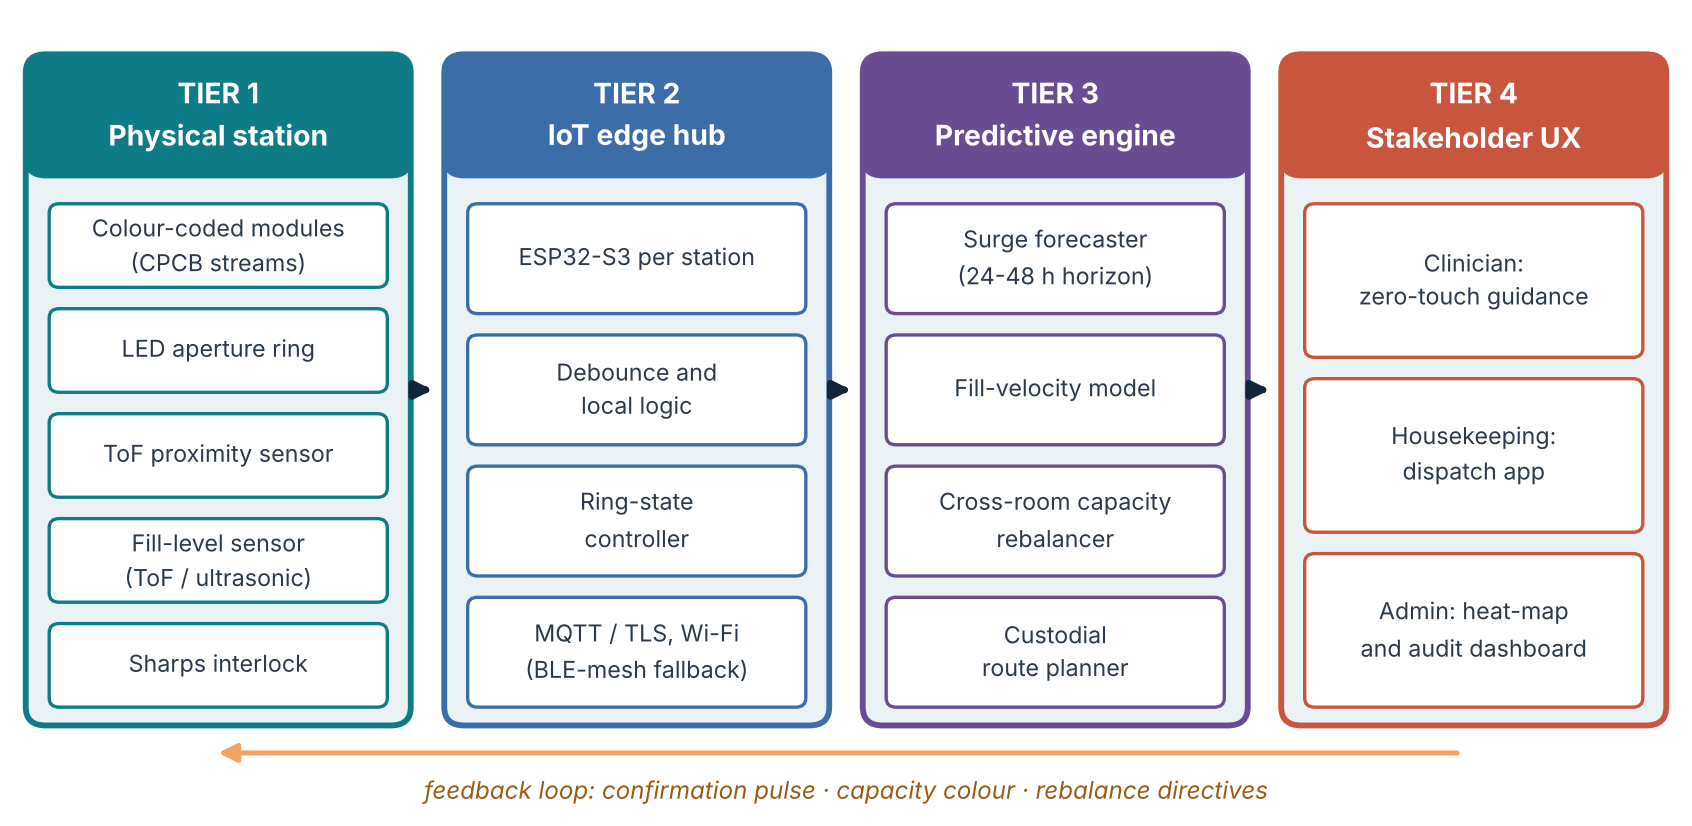
\includegraphics[width=0.66\textwidth]{fig/fig_arch.png}
\caption{Proposed four-tier architecture. Data flows right; confirmation, capacity colour and rebalancing directives flow back to the station.}\label{fig:arch}
\end{figure*}

\subsection{Feature A: Surge forecasting (Phase 2)}
Our finding that peaks are not clock-driven argues for forecasting, but we do not claim a model. We would begin with a seasonal-naive or calendar baseline (campus events, camps, exam weeks), which forecasting practice recommends before anything complex \cite{hyndman2021}, and move to Prophet or an LSTM only if logs justify it \cite{taylor2018,hochreiter1997}. At roughly 100--150 daily visitors an LSTM is likely excessive, and fill velocity $v=\Delta V/\Delta t$ is simple arithmetic; the value is in the \emph{decision}, not the maths. The administrator would see a one-line alert at the start of the day (\figref{fig:ui}b).

\subsection{Feature B: Fill sensing and rebalancing (Phase 1)}
Each module reports fill level, and a lid-opening counter gives a second signal of use. In the sample-room corner of \figref{fig:overflow}, even simple per-bin thresholds would have flagged bucket~1 before it was heaped and shown that bucket~3 had spare capacity. Because modules are identical, rebalancing means lifting a spare from a quiet room, not buying one.

\subsection{Feature C: Point-of-disposal guidance (Phase 1)}
Each aperture has a diffused LED ring and a narrow-beam time-of-flight sensor (\figref{fig:station}). \textbf{Ambient:} a dim glow (green below 50\% fill, amber 50--80\%, red above 80\%). \textbf{Approach} (hand within about 60~cm): the ring shows the module's BMW colour, a nudge at the point of choice \cite{thaler2008}. \textbf{Confirmation:} one green pulse after the drop; an amber double-flash if the module is near capacity or the drop looks wrong. Colour is lit only on approach to avoid alarm fatigue \cite{sendelbach2013}; an optional chime has a mute and a night mode \cite{wickens2013}; pictogram and position repeat the colour for colour-blind users \cite{birch2012}; a dark bezel keeps the white sharps ring above the 3:1 contrast level \cite{wcag2018}.
\begin{figure*}[!t]
\centering
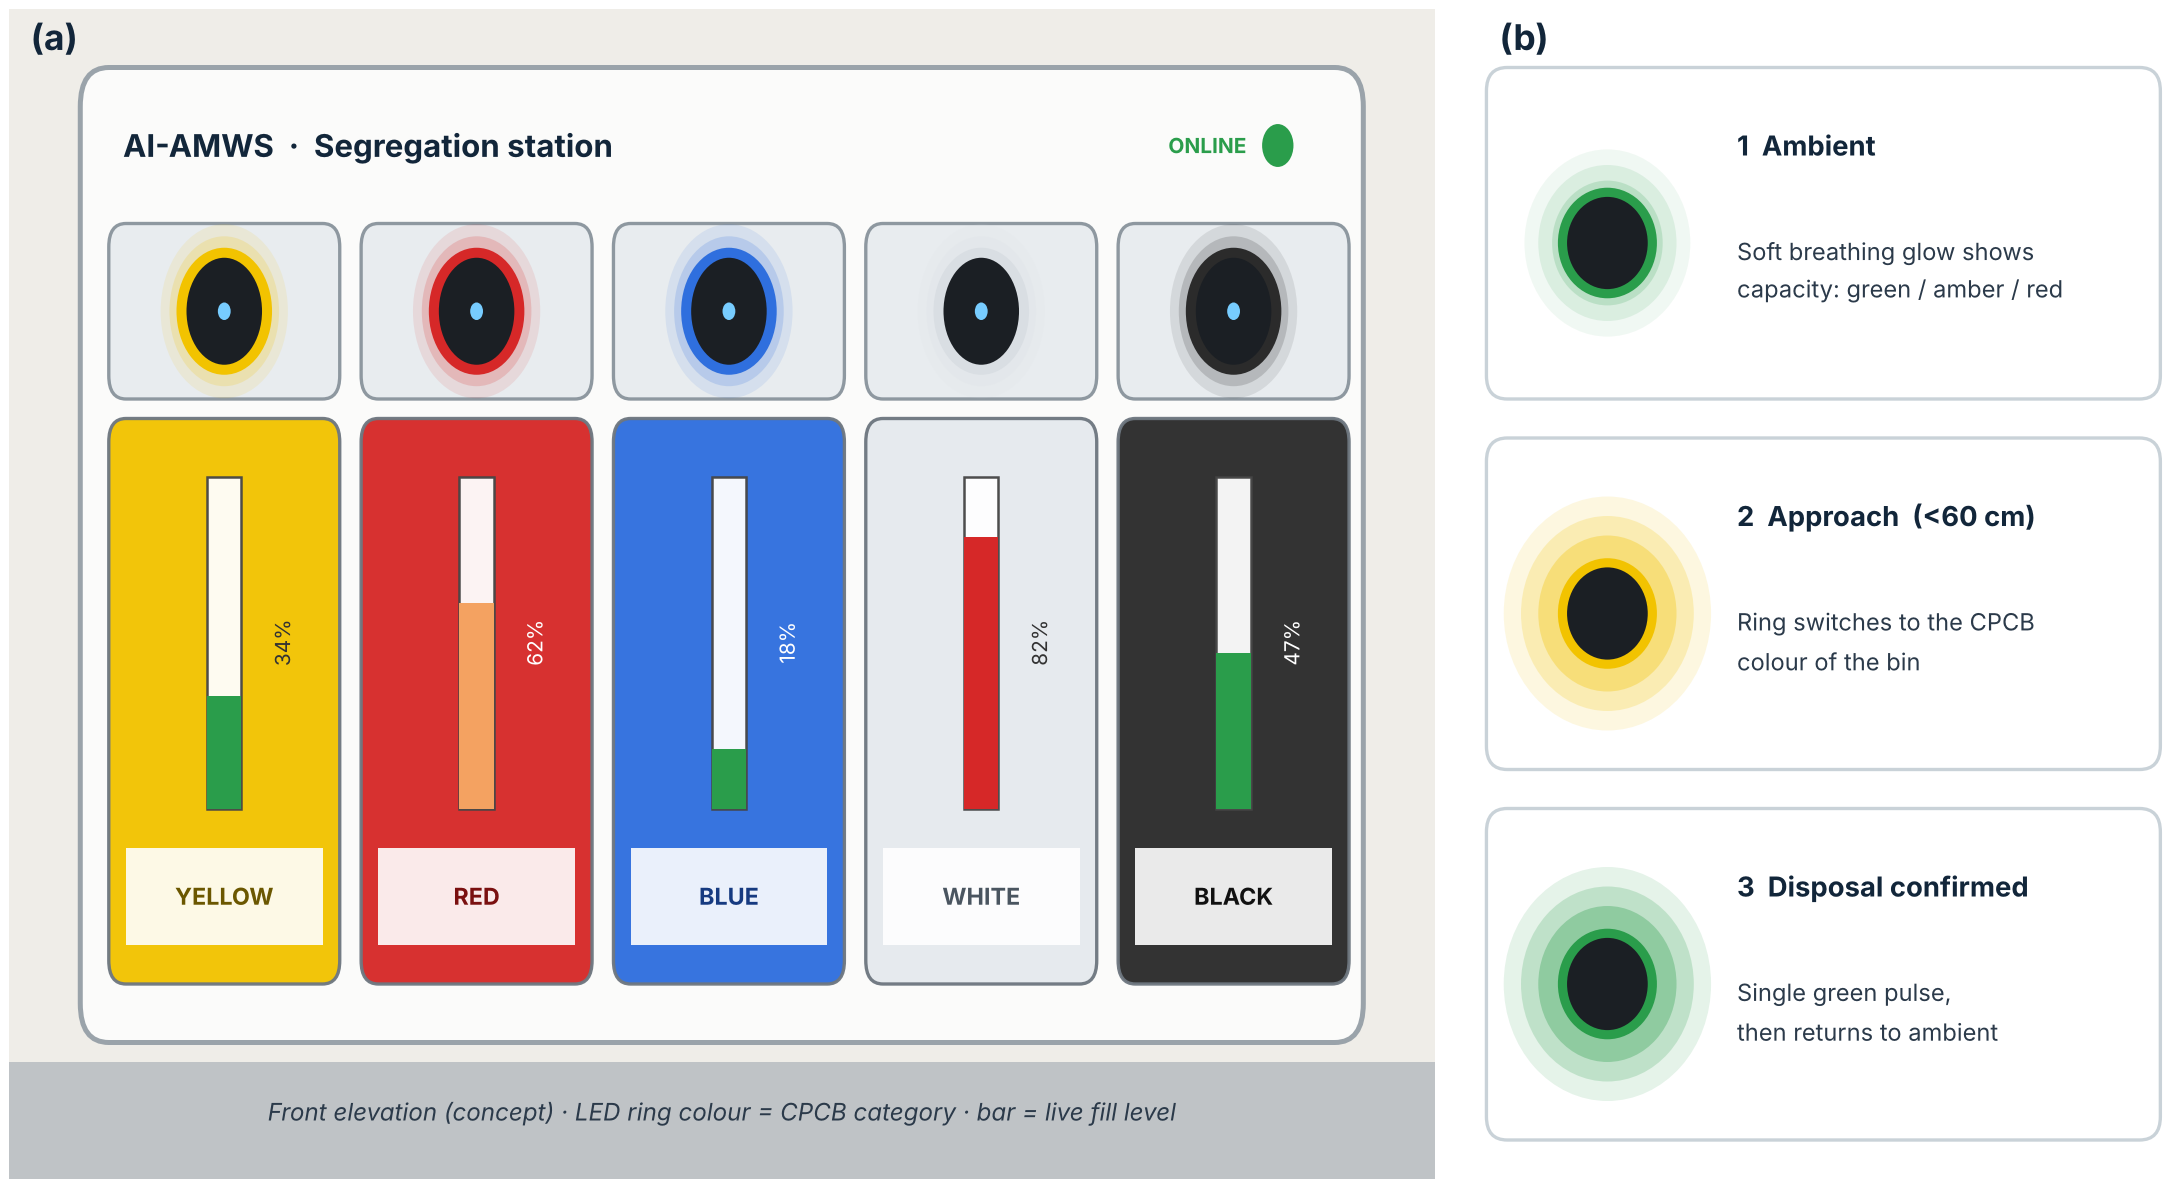
\includegraphics[width=0.74\textwidth]{fig/fig_station.png}
\caption{Concept of the proposed station. (a) Front elevation with five modules; (b) the three ring states. Illustrative render by the group, not a built prototype.}\label{fig:station}
\end{figure*}

\subsection{Feature D: Need-based dispatch (Phase 2)}
Housekeepers would get a ranked list in a mobile web app (\figref{fig:ui}a). Two rules set urgency: 75\% fill, and a holding limit. The BMW Rules allow 48 hours for untreated waste \cite{bmw2016}; with external collection occurring on a 72-hour cycle, local buffer accumulation demands proactive containment. We suggest a stricter 12-hour in-room target as an internal operational choice management can configure. Routing is a small travelling-salesperson problem over the rooms that breach either rule. The dashboard (\figref{fig:ui}b) adds a heat-map and an audit log with simple flags (a module filling far faster than its siblings, lid openings with no fill change, a sharps-interlock override).
\begin{figure*}[!t]
\centering
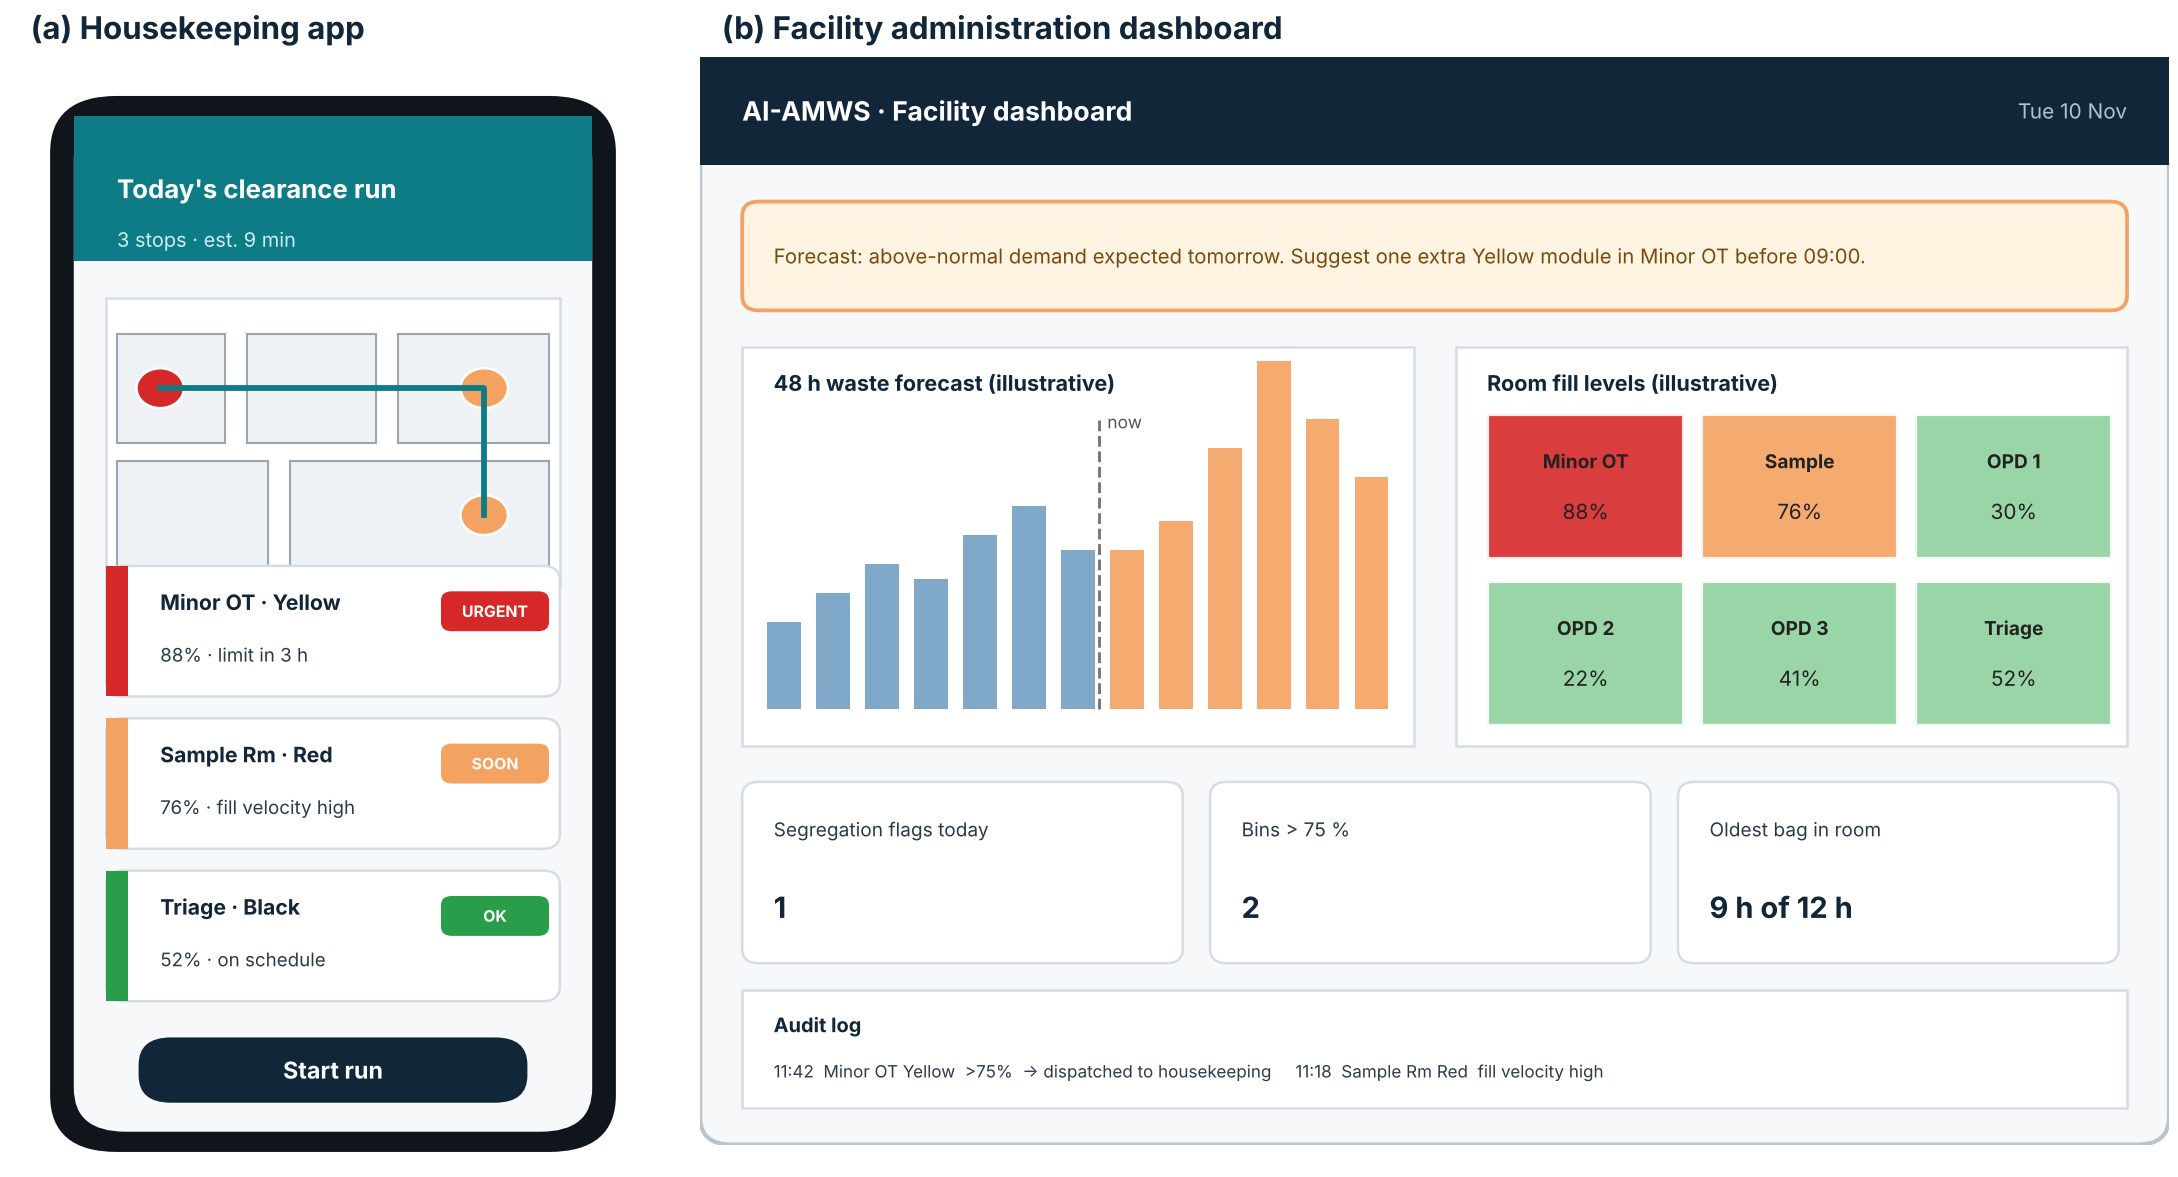
\includegraphics[width=0.74\textwidth]{fig/fig_ui.png}
\caption{Stakeholder interface concepts: (a) housekeeping app; (b) administrator dashboard. Values are illustrative placeholders for layout, not measured data.}\label{fig:ui}
\end{figure*}

\subsection{Spatial placement}
On the plan we marked in the field we suggest two tiers (\figref{fig:plans}B): point-of-care stations (red) beside cots, dressing trolleys and sample chairs, and public or general-waste stations (green) at the lounge, entry and desks. This follows R6 and Norman's principle of mapping. It is a sketch from our reading of the workflow; reach distances were not measured.
\begin{figure*}[!t]
\centering
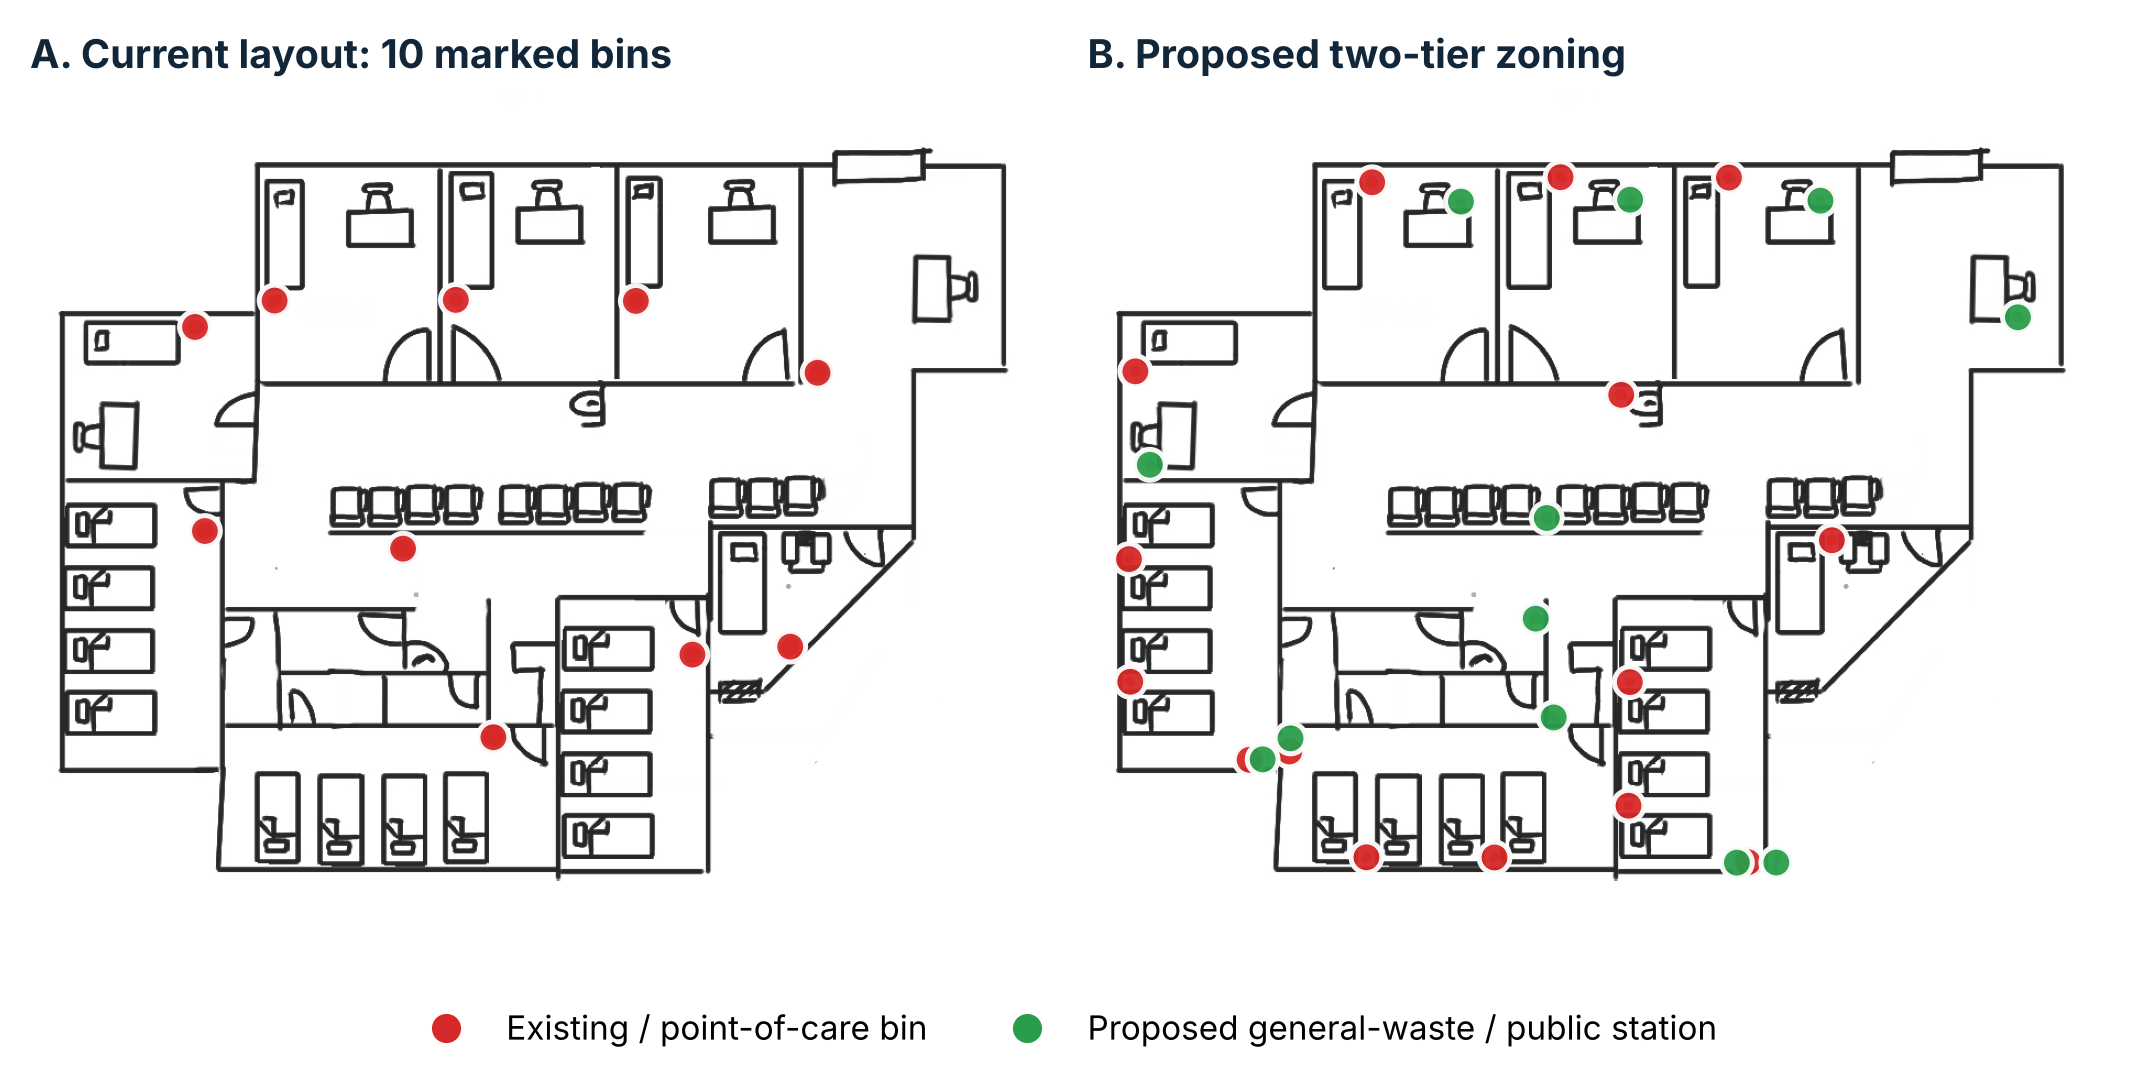
\includegraphics[width=0.70\textwidth]{fig/fig_plans.png}
\caption{Floor-plan overlay. (A) Bin positions as marked in the field; (B) suggested two-tier zoning. Markers enlarged for legibility.}\label{fig:plans}
\end{figure*}

\subsection{Technical risks and mitigations}
\textbf{False triggers:} staff walking past could light a ring; a narrow beam aimed at the aperture, a short dwell requirement and a brightness cap reduce this, and thresholds would need on-site tuning. \textbf{Fouling and disinfection:} sensors must be sealed and wipeable, with a self-test that flags faults, since a sensor that fails silently is worse than none. \textbf{Maintenance and cost:} every electronic part needs an owner and spares; we give no cost figure and recommend vendor quotes before Phase~1. \textbf{Connectivity:} rings work from local logic offline, with a BLE-mesh relay. \textbf{Privacy:} no cameras in Phase~1; item verification by camera is deferred pending consent and review.

% ================= 8 EVALUATION =================
\section{Analytic Evaluation and Grounding}
\subsection{What kind of evaluation this is}
We did not prototype or test with users, so there is no usability data for AI-AMWS. Our evaluation is \emph{analytic}: a scenario-based heuristic evaluation (\tabref{tab:heur}) over three scenarios (S1: a nurse discards a dressing mid-procedure; S2: a patient discards a wrapper in the lounge; S3: a housekeeper responds to an alert), and the grounding in \tabref{tab:ground}. This shows that each decision is \emph{reasoned and supported}, not that it \emph{works}.
\begin{table*}[!t]
\centering\footnotesize
\caption{Grounding of design decisions: field evidence, published support, and what remains unvalidated.}\label{tab:ground}
\begin{tabularx}{\textwidth}{@{}>{\bfseries}p{3.2cm} p{1.6cm} Y Y@{}}
\toprule
Decision & Field & Published support & Still to validate\\\midrule
Category colour at the aperture on approach & F2, F4 & Nudges at the point of choice \cite{thaler2008}; signifiers \cite{norman2013} & Glance time and wrong-bin rate on a mock-up\\
Standard lidded modules, shaped apertures & F2, F3 & Error-proofing beats rules \cite{shingo1986}; BMW container rules \cite{bmw2016} & Reach and one-handed use\\
Success pulse and amber flag & F2 & Gulf of evaluation \cite{norman2013} & Whether feedback lowers errors\\
Colour only on approach; optional muted chime & -- & Alarm fatigue \cite{sendelbach2013,wickens2013} & Acceptable brightness in quiet wards\\
Pictogram, position, dark bezel & F5 & Colour deficiency \cite{birch2012}; 3:1 contrast \cite{wcag2018}; our 1.9:1 yellow sample & Contrast with a reference card\\
Fill sensing, rebalancing & F2, F6 & Fill sensing established \cite{medvedev2015}; 48-h limit \cite{bmw2016} & Sensor accuracy in the rooms\\
Calendar baseline before ML forecast & F6 & Simple baselines first \cite{hyndman2021,taylor2018} & Weeks of fill logs\\
Need-based dispatch & F6 & Holding limit \cite{bmw2016} & Housekeeper interviews\\
Phase 0 first & F1--F3 & Reviews of Indian practice stress segregation at source \cite{datta2018,capoor2017} & Residual error after Phase 0\\
\bottomrule
\end{tabularx}
\end{table*}

\subsection{How validation would be done}
Low-fidelity prototypes can expose most interface problems cheaply \cite{rettig1994}, and a handful of participants finds a large share of usability problems in a round \cite{virzi1992}. We would build a 1:1 foam and card mock-up of one station and have 5--8 staff and students perform S1--S3, recording hesitation, wrong-bin choices and comments against the present buckets. Medical-device usability standards such as IEC~62366-1 \cite{iec62366} set out a fuller process, though bins are not medical devices. We state this as a plan, not as work done.

% ================= 9 DISCUSSION =================
\section{Discussion and Reflection}
\subsection{Trade-offs}
\textbf{Durability versus intelligence:} electronics in a disinfected clinic must be sealed, so a low-tech first step is wiser. \textbf{Over-automation:} forecasts can be wrong, so humans must be able to override. \textbf{Title and claims:} we call the concept ``AI-AMWS'' for continuity, but the intelligence is modest and late; the early value is standardisation and feedback.

\subsection{Method self-critique}
We spent one visit, so we saw a snapshot rather than a surge. Observers change behaviour, and the evidence on such effects is mixed rather than absent \cite{mccambridge2014}, so staff may have tidied up or answered diplomatically. We recorded what staff \emph{said} about peaks and logistics and did not time them. Photographs show what was there once. The contrast values come from one photograph under uncontrolled lighting. The baseline is secondary data, so old-versus-new differences are indicative. The heuristic ratings are ours, and the stakeholder views are inferred. We did not interview patients or housekeepers directly. These limits are why we ground rather than claim.

\subsection{What surprised us, and what we would change}
We expected some improvement inside the rooms and found instead the contrast between an excellent buffer rack and improvised buckets beside it. The institution knows what a good bin looks like, but nobody owned the point of care. The paint story was a second surprise: a sensible fix whose benefit depends on bin colour. Next time we would use a grey reference card and lux meter, observe on several days, shadow one clearance run with consent, and measure cot-to-bin distances.

\subsection{The attentive engineer}
Clinicians are not the problem. The design question is how to make the safe action the easy one when attention is elsewhere. This shift from ``training problem'' to ``environment problem'' is the main lesson we take away.

% ================= 10 CONCLUSION =================
\section{Conclusion}
The renovation improved the building and added a good external buffer, but waste handling inside the rooms still depends on memory, briefings and phone calls. We documented this with photographs, a hand-drawn plan, a receptacle checklist, a contrast sample and staff statements; interpreted it through Norman, Rasmussen and Reason; and suggested a staged evolution, starting with low-cost standardisation and adding guidance, sensing and forecasting only as evidence supports them. We did not build or test the proposal; every decision is instead tied to field evidence and published research, with its open questions listed. Future work: a mock-up test with real staff, a four-week fill log, a measured reach audit, and independent evaluators for the heuristic ratings.

\section*{Acknowledgements}
We thank the Medical Centre staff for their time and candour, and Prof.\ Guimar\~aes for guidance on scope.

\begin{thebibliography}{99}\fontsize{8}{9.4}\selectfont
\setlength{\itemsep}{0pt}
\bibitem{who2014} Y.\ Chartier \emph{et al.}, \emph{Safe Management of Wastes from Health-Care Activities}, 2nd~ed. Geneva: WHO, 2014.
\bibitem{bmw2016} MoEFCC, Govt.\ of India, ``Bio-Medical Waste Management Rules, 2016,'' G.S.R.~343(E), Mar.~2016.
\bibitem{prusstun2005} A.\ Pr\"uss-\"Ust\"un, E.\ Rapiti and Y.\ Hutin, ``Estimation of the global burden of disease attributable to contaminated sharps injuries among health-care workers,'' \emph{Am.\ J.\ Ind.\ Med.}, vol.~48, no.~6, pp.~482--490, 2005.
\bibitem{datta2018} P.\ Datta, G.\ K.\ Mohi and J.\ Chander, ``Biomedical waste management in India: Critical appraisal,'' \emph{J.\ Lab.\ Physicians}, vol.~10, no.~1, pp.~6--14, 2018.
\bibitem{capoor2017} M.\ R.\ Capoor and K.\ T.\ Bhowmik, ``Current perspectives on biomedical waste management: Rules, conventions and treatment technologies,'' \emph{Indian J.\ Med.\ Microbiol.}, vol.~35, no.~2, pp.~157--164, 2017.
\bibitem{norman2013} D.\ A.\ Norman, \emph{The Design of Everyday Things}, rev.\ ed. New York: Basic Books, 2013.
\bibitem{bmw2018} MoEFCC, Govt.\ of India, ``Bio-Medical Waste Management (Amendment) Rules, 2018,'' G.S.R.~234(E), Mar.~2018.
\bibitem{swm2016} MoEFCC, Govt.\ of India, ``Solid Waste Management Rules, 2016,'' G.S.R.~371(E), Apr.~2016.
\bibitem{norman1986} D.\ A.\ Norman, ``Cognitive engineering,'' in \emph{User Centered System Design}, D.\ A.\ Norman and S.\ W.\ Draper, Eds. Hillsdale, NJ: Erlbaum, 1986, pp.~31--61.
\bibitem{rasmussen1983} J.\ Rasmussen, ``Skills, rules, and knowledge; signals, signs, and symbols, and other distinctions in human performance models,'' \emph{IEEE Trans.\ Syst., Man, Cybern.}, vol.~SMC-13, no.~3, pp.~257--266, 1983.
\bibitem{reason1990} J.\ Reason, \emph{Human Error}. Cambridge, U.K.: Cambridge Univ.\ Press, 1990.
\bibitem{reason2000} J.\ Reason, ``Human error: models and management,'' \emph{BMJ}, vol.~320, no.~7237, pp.~768--770, 2000.
\bibitem{thaler2008} R.\ H.\ Thaler and C.\ R.\ Sunstein, \emph{Nudge}. New Haven, CT: Yale Univ.\ Press, 2008.
\bibitem{shingo1986} S.\ Shingo, \emph{Zero Quality Control: Source Inspection and the Poka-Yoke System}. Cambridge, MA: Productivity Press, 1986.
\bibitem{sendelbach2013} S.\ Sendelbach and M.\ Funk, ``Alarm fatigue: a patient safety concern,'' \emph{AACN Adv.\ Crit.\ Care}, vol.~24, no.~4, pp.~378--386, 2013.
\bibitem{wickens2013} C.\ D.\ Wickens, J.\ D.\ Lee, Y.\ Liu and S.\ Gordon-Becker, \emph{Introduction to Human Factors Engineering}, 2nd~ed. Harlow, U.K.: Pearson, 2013.
\bibitem{birch2012} J.\ Birch, ``Worldwide prevalence of red-green color deficiency,'' \emph{J.\ Opt.\ Soc.\ Am.\ A}, vol.~29, no.~3, pp.~313--320, 2012.
\bibitem{wcag2018} W3C, ``Web Content Accessibility Guidelines (WCAG) 2.1,'' W3C Recommendation, Jun.~2018.
\bibitem{medvedev2015} A.\ Medvedev \emph{et al.}, ``Waste management as an IoT-enabled service in smart cities,'' in \emph{Internet of Things, Smart Spaces, and Next Generation Networks and Systems} (LNCS 9247). Springer, 2015.
\bibitem{hyndman2021} R.\ J.\ Hyndman and G.\ Athanasopoulos, \emph{Forecasting: Principles and Practice}, 3rd~ed. Melbourne: OTexts, 2021.
\bibitem{taylor2018} S.\ J.\ Taylor and B.\ Letham, ``Forecasting at scale,'' \emph{Amer.\ Statistician}, vol.~72, no.~1, pp.~37--45, 2018.
\bibitem{g8report} Group~8, ``Attentive Segregation: A UX-Driven IoT-Assisted System for Improving Medical Waste Management at IIT Gandhinagar,'' FUX course project report, IIT Gandhinagar, previous cohort, unpublished.
\bibitem{beyer1998} H.\ Beyer and K.\ Holtzblatt, \emph{Contextual Design}. San Francisco, CA: Morgan Kaufmann, 1998.
\bibitem{braun2006} V.\ Braun and V.\ Clarke, ``Using thematic analysis in psychology,'' \emph{Qual.\ Res.\ Psychol.}, vol.~3, no.~2, pp.~77--101, 2006.
\bibitem{nielsen1990} J.\ Nielsen and R.\ Molich, ``Heuristic evaluation of user interfaces,'' in \emph{Proc.\ ACM CHI}, Seattle, WA, 1990, pp.~249--256.
\bibitem{nielsen1994} J.\ Nielsen, ``Enhancing the explanatory power of usability heuristics,'' in \emph{Proc.\ ACM CHI}, Boston, MA, 1994, pp.~152--158.
\bibitem{nielsen1993} J.\ Nielsen, \emph{Usability Engineering}. San Diego, CA: Academic Press, 1993.
\bibitem{hochreiter1997} S.\ Hochreiter and J.\ Schmidhuber, ``Long short-term memory,'' \emph{Neural Comput.}, vol.~9, no.~8, pp.~1735--1780, 1997.
\bibitem{rettig1994} M.\ Rettig, ``Prototyping for tiny fingers,'' \emph{Commun.\ ACM}, vol.~37, no.~4, pp.~21--27, 1994.
\bibitem{virzi1992} R.\ A.\ Virzi, ``Refining the test phase of usability evaluation: how many subjects is enough?'' \emph{Hum.\ Factors}, vol.~34, no.~4, pp.~457--468, 1992.
\bibitem{iec62366} IEC, ``IEC 62366-1:2015 Medical devices --- Part 1: Application of usability engineering to medical devices,'' 2015.
\bibitem{mccambridge2014} J.\ McCambridge, J.\ Witton and D.\ R.\ Elbourne, ``Systematic review of the Hawthorne effect: new concepts are needed to study research participation effects,'' \emph{J.\ Clin.\ Epidemiol.}, vol.~67, no.~3, pp.~267--277, 2014.

\end{thebibliography}

\end{document}
